\documentclass[10pt,a4paper]{article}

\usepackage[utf8]{inputenc}
\usepackage[english]{babel}
\usepackage[english]{isodate}
\usepackage[parfill]{parskip}
\usepackage{graphicx}

\usepackage{listings}
\usepackage{color}
\definecolor{dkgreen}{rgb}{0,0.6,0}
\definecolor{gray}{rgb}{0.5,0.5,0.5}
\definecolor{mauve}{rgb}{0.58,0,0.82}
\lstset{frame=tb,
  language=C,
  aboveskip=3mm,
  belowskip=3mm,
  showstringspaces=false,
  columns=flexible,
  basicstyle={\small\ttfamily},
  numbers=none,
  numberstyle=\tiny\color{gray},
  keywordstyle=\color{blue},
  commentstyle=\color{dkgreen},
  stringstyle=\color{mauve},
  breaklines=true,
  breakatwhitespace=true
  tabsize=3
}

\title{User Guide for Developing a Virtual Object Layer Plugin}
\author{Mohamad Chaarawi}

\begin{document}

\maketitle

\newpage
\pagenumbering{Roman}
\tableofcontents
\newpage

\pagenumbering{arabic}


%%% Local Variables: 
%%% mode: latex
%%% TeX-master: t
%%% End: 

\section{Introduction}
The Virtual Object Layer (VOL) is an abstraction layer in the HDF5
library that intercepts all API calls that could potentially access
objects in an HDF5 container and forwards those calls to plugin
``object drivers''. The plugins could store the objects in variety of
ways. A plugin could, for example, have objects be distributed
remotely over different platforms, provide a raw mapping of the model
to the file system, or even store the data in other file formats (like
native netCDF or HDF4 format). The user still gets the same data model
where access is done to a single HDF5 “container”; however the plugin
object driver translates from what the user sees to how the data is
actually stored. Having this abstraction layer maintains the object
model of HDF5 and would allow HDF5 developers or users to write their
own plugins for accessing HDF5 data.

This user guide is for developers interested in developing a VOL
plugin for the HDF5 library. The document is meant to be used in
conjunction with the HDF5 reference manual. It is assumed that the
reader has good knowledge of the VOL architecture obtained by reading
the VOL architectural design document ~\ref{HERE} MSC-ref. The
document will cover the steps needed to create external and internal
VOL plugins. Both ways have a lot of common steps and rules that will
be covered first.

\section{Creating a VOL Plugin}
\label{sec:vol}
Each VOL plugin should be of type {\tt H5VL\_class\_t} that is defined
as:

\begin{lstlisting}
/* Class information for each VOL driver */
typedef struct H5VL_class_t {
    H5VL_class_value_t value;
    const char *name;
    herr_t  (*initialize)(void);
    herr_t  (*terminate)(void);
    size_t  info_size;
    void *  (*fapl_copy)(const void *info);
    herr_t  (*fapl_free)(void *info);
    H5VL_attr_class_t          attr_cls;
    H5VL_datatype_class_t      datatype_cls;
    H5VL_dataset_class_t       dataset_cls;
    H5VL_file_class_t          file_cls;
    H5VL_group_class_t         group_cls;
    H5VL_link_class_t          link_cls;
    H5VL_object_class_t        object_cls;
    H5VL_async_class_t         async_cls;
} H5VL_class_t;
\end{lstlisting}

The {\tt value} field is an integer enum identifier that should be
greater than 128 for external plugins and smaller than 128 for
internal plugins. This plugin identifier is used to select the VOL
plugin to be used when creating/accessing the HDF5 container in the
application. Setting it in the VOL structure is required.

The {\tt name} field is a string that identifies the VOL plugin
name. Setting it is not required.

The {\tt initialize} field is a function pointer - MSC not used now!.

The {\tt terminate} field is a function pointer - MSC not used now!.

The {\tt info\_size} field indicates the size required to store the
info data that the plugin needs. That info data is passed when the
plugin is selected for usage with the file access property list (fapl)
function. It might be that the plugin defined does not require any
information from the user, which means the size in this field will be
zero. More information about the info data and the fapl selection
routines follow later.

The {\tt fapl\_copy} field is a function pointer that is called when
the plugin is selected with the fapl function. It allows the plugin to
make a copy if the info data since the user might free it when closing
the fapl. It is required if there is info data needed by the plugin.

The {\tt fapl\_free} field is a function pointer that is called to
free the info data when the fapl close routine is called. It is
required if there is info data needed by the plugin.

The rest of the fields in the {\tt H5VL\_class\_t} struct are
``subclasses'' that define all the object VOL function callbacks that
are mapped to from the HDF5 API layer and will be detailed in the
following sub-sections.

\subsection{Mapping the API to the Callbacks}
\label{sec:map}

The callback interface defined for the VOL has to be general enough to
handle all the HDF5 API operations that would access the
file. Furthermore it has to capture future additions to the HDF5
library with little to no changes to the callback interface. Changing
the interface often whenever new features are added would be
discouraging to plugin developers since that would mean reworking
their VOL plugin structure. To remedy this issue, every callback will
contain two parameters:
\begin{itemize}
\item A data transfer property list (DXPL) which allows that API to
  put some properties on for the plugins to retrieve if they have to
  for particular operations, without having to add arguments to the
  VOL callback function.
\item A pointer to a request ({\tt void **req}) to handle asynchronous
  operations if the HDF5 library adds support for them in future
  releases (beyond the 1.8 series). That pointer is set by the VOL
  plugin to a request object it creates to manage progress on that
  asynchronous operation. If the {\tt req} is {\tt NULL}, that means
  that the API operation is blocking and so the plugin would not
  execute the operation asynchronously. If the plugin does not support
  asynchronous operations, it needs not to worry about this field and
  leaves it unset.
\end{itemize}

In order to keep the number of the VOL object classes and callbacks
concise and readable, it was decided to not have a one-to-one mapping
between API operation and callbacks. Furthermore, to keep the
callbacks themselves short and not cluttered with a lot of parameters,
some of the parameters are passed in as properties in property lists
included with the callback. The value of those properties can be
retrieved by calling the public routine (or its private version if
this is an internal plugin): 
\begin{lstlisting}
herr_t H5Pget(hid_t plist_id, const char *property_name, void *value);
\end{lstlisting}
The property names and value types will be detailed when describing
each callback in their respective sections.

The HDF5 library provides several routines to access an object in the
container. For example to open an attribute on a group object, the
user could use {\tt H5Aopen()} and pass the group identifier directly
where the attribute needs to be opened. Alternatively, the user could
use {\tt H5Aopen\_by\_name()} or {\tt H5Aopen\_by\_idx()} to open the
attribute, which provides a more flexible way of locating the
attribute, whether by a starting object location and a path or an
index type and traversal order. All those types of accesses usually
map to one VOL callback with a parameter that indicates the access
type. In the example of opening an attribute, the three API open
routine will map to the same VOL open callback but with a different
location parameter. The same applies to all types of routines that
have multiple types of accesses.  The location parameter is a
structure defined as follows:

\begin{lstlisting}
/* 
 * Structure to hold parameters for object locations.
 * either: BY_ID, BY_NAME, BY_IDX, BY_ADDR, BY_REF 
 */

typedef struct H5VL_loc_params_t {
    H5I_type_t obj_type; /* The object type of the location object */
    H5VL_loc_type_t type; /* The location type */
    union { /* parameters of the location */
        struct H5VL_loc_by_name loc_by_name;
        struct H5VL_loc_by_idx  loc_by_idx;
        struct H5VL_loc_by_addr loc_by_addr;
        struct H5VL_loc_by_ref  loc_by_ref;
    }loc_data;
} H5VL_loc_params_t

/* 
 * Types for different ways that objects are located in an 
 * HDF5 container.
 */
typedef enum H5VL_loc_type_t {
    /* starting location is the target object*/
    H5VL_OBJECT_BY_SELF, 

    /* location defined by object and path in H5VL_loc_by_name */
    H5VL_OBJECT_BY_NAME, 

    /* location defined by object, path, and index in H5VL_loc_by_idx */
    H5VL_OBJECT_BY_IDX,

    /* location defined by physical address in H5VL_loc_by_addr */
    H5VL_OBJECT_BY_ADDR,

    /* NOT USED */
    H5VL_OBJECT_BY_REF
} H5VL_loc_type_t;

struct H5VL_loc_by_name {
    const char *name; /* The path relative to the starting location */
    hid_t plist_id; /* The link access property list */
};

struct H5VL_loc_by_idx {
    const char *name; /* The path relative to the starting location */
    H5_index_t idx_type; /* Type of index */
    H5_iter_order_t order; /* Index traversal order */
    hsize_t n; /* position in index */
    hid_t plist_id; /* The link access property list */
};

struct H5VL_loc_by_addr {
    haddr_t addr; /* physical address of location */
};

/* Not used for now */
struct H5VL_loc_by_ref {
    H5R_type_t ref_type;
    const void *_ref;
    hid_t plist_id;
};
\end{lstlisting}

Another large set of operations that would make a one-to-one mapping
difficult are the {\tt Get} operations that retrieve something from an
object; for example a property list or a datatype of a dataset,
etc... To handle that, each class of objects has a general get
callback with a {\tt get\_type} and a {\tt va\_list} argument to handle
the multiple get operations. More information about types and the
arguments for each type will be detailed in the corresponding class
arguments.

Finally there are a set of functions for the file and general object
(H5O) classes that are not widely used or interesting enough for
plugin developers to implement. Those routines are mapped to a {\tt
  misc} callback in their respective class.

\subsection{The Attribute Function Callbacks}
The attribute API routines (H5A) allow HDF5 users to create and manage
HDF5 attributes. All the H5A API routines that modify the HDF5
container map to one of the attribute callback routines in this
class that the plugin needs to implement:

\begin{lstlisting}
typedef struct H5VL_attr_class_t {
    void *(*create)(void *obj, H5VL_loc_params_t loc_params, 
        const char *attr_name, hid_t acpl_id, hid_t aapl_id, 
        hid_t dxpl_id, void **req);

    void *(*open)(void *obj, H5VL_loc_params_t loc_params, 
        const char *attr_name, hid_t aapl_id, hid_t dxpl_id, void **req);

    herr_t (*read)(void *attr, hid_t mem_type_id, void *buf, 
        hid_t dxpl_id, void **req);

    herr_t (*write)(void *attr, hid_t mem_type_id, const void *buf, 
        hid_t dxpl_id, void **req);

    herr_t (*iterate)(void *obj, H5VL_loc_params_t loc_params,
        H5_index_t idx_type, H5_iter_order_t order, hsize_t *n, 
        H5A_operator2_t  op, void *op_data, hid_t dxpl_id, void **req);

    herr_t (*get)(void *obj, H5VL_attr_get_t get_type, hid_t dxpl_id, 
        void **req, va_list arguments);

    herr_t (*remove)(void *obj, H5VL_loc_params_t loc_params, 
        const char *attr_name, hid_t dxpl_id, void **req);

    herr_t (*close)(void *attr, hid_t dxpl_id, void **req);
} H5VL_attr_class_t;
\end{lstlisting}

The {\tt create} callback in the attribute class should create an
attribute object in the container of the location object and
returns a pointer to the attribute structure containing information to
access the attribute in future calls. 

\textbf{Signature:}
\begin{lstlisting}
    void *(*create)(void *obj, H5VL_loc_params_t loc_params, 
        const char *attr_name, hid_t acpl_id, hid_t aapl_id, 
        hid_t dxpl_id, void **req);
\end{lstlisting}

\textbf{Arguments:}\\
\begin{tabular}{l p{10cm}}
  {\tt obj} & (IN): Pointer to an object where the attribute needs
  to be created or where the look-up of the target object needs to
  start.\\
  {\tt loc\_params} & (IN): The location parameters as explained in
  section~\ref{sec:map}.\\
  {\tt attr\_name} & (IN): The name of the attribute to be created.\\
  {\tt acpl\_id} & (IN): The attribute creation property list. It contains
  all the attribute creation properties in addition to the attribute
  datatype (an {\tt hid\_t}) and dataspace (an {\tt hid\_t}) that can
  be retrieved with the properties, {\tt H5VL\_ATTR\_TYPE\_ID} and
  {\tt H5VL\_ATTR\_SPACE\_ID}.\\
  {\tt aapl\_id} & (IN): The attribute access property list.\\
  {\tt dxpl\_id} & (IN): The data transfer property list.\\
  {\tt req} & (IN/OUT): A pointer to the asynchronous request of the
  operation created by the plugin.\\
\end{tabular}

The {\tt open} callback in the attribute class should open an
attribute object in the container of the location object and returns a
pointer to the attribute structure containing information to access
the attribute in future calls. 

\textbf{Signature:}
\begin{lstlisting}
    void *(*open)(void *obj, H5VL_loc_params_t loc_params, 
        const char *attr_name, hid_t aapl_id, hid_t dxpl_id, void **req);
\end{lstlisting}

\textbf{Arguments:}\\
\begin{tabular}{l p{10cm}}
  {\tt obj} & (IN): Pointer to an object where the attribute needs to be
  opened or where the look-up of the target object needs to start.\\
  {\tt loc\_params} & (IN): The location parameters as explained in
  section~\ref{sec:map}.\\
  {\tt attr\_name} & (IN): The name of the attribute to be opened.\\
  {\tt aapl\_id} & (IN): The attribute access property list.\\
  {\tt dxpl\_id} & (IN): The data transfer property list.\\
  {\tt req} & (IN/OUT): A pointer to the asynchronous request of the
  operation created by the plugin.\\
\end{tabular}

The {\tt read} callback in the attribute class should read data from
the attribute object and returns an {\tt herr\_t} indicating success or
failure.

\textbf{Signature:}
\begin{lstlisting}
    herr_t (*read)(void *attr, hid_t mem_type_id, void *buf, 
        hid_t dxpl_id, void **req);
\end{lstlisting}

\textbf{Arguments:}\\
\begin{tabular}{l p{10cm}}
  {\tt attr} & (IN): Pointer to the attribute object.\\
  {\tt mem\_type\_id} & (IN): The memory datatype of the attribute.\\
  {\tt buf} & (OUT): Data buffer to be read into.\\
  {\tt dxpl\_id} & (IN): The data transfer property list.\\
  {\tt req} & (IN/OUT): A pointer to the asynchronous request of the
  operation created by the plugin.\\
\end{tabular}

The {\tt write} callback in the attribute class should write data to
the attribute object and returns an {\tt herr\_t} indicating success or
failure.

\textbf{Signature:}
\begin{lstlisting}
    herr_t (*write)(void *attr, hid_t mem_type_id, const void *buf, 
        hid_t dxpl_id, void **req);
\end{lstlisting}

\textbf{Arguments:}\\
\begin{tabular}{l p{10cm}}
  {\tt attr} & (IN): Pointer to the attribute object.\\
  {\tt mem\_type\_id} & (IN): The memory datatype of the attribute.\\
  {\tt buf} & (IN): Data buffer to be written.\\
  {\tt dxpl\_id} & (IN): The data transfer property list.\\
  {\tt req} & (IN/OUT): A pointer to the asynchronous request of the
  operation created by the plugin.\\
\end{tabular}

The {\tt iterate} callback in the attribute class should iterate over
the attributes in the container of the location object and call the
user defined function on each one. It returns an {\tt herr\_t}
indicating success or failure.

\textbf{Signature:}
\begin{lstlisting}
    herr_t (*iterate)(void *obj, H5VL_loc_params_t loc_params,
        H5_index_t idx_type, H5_iter_order_t order, hsize_t *n, 
        H5A_operator2_t  op, void *op_data, hid_t dxpl_id, void **req);
\end{lstlisting}

\textbf{Arguments:}\\
\begin{tabular}{l p{10cm}}
  {\tt obj} & (IN): Pointer to an object where the iteration needs
  to happen or where the look-up of the target object needs to
  start.\\
  {\tt loc\_params} & (IN): The location parameters as
  explained in section~\ref{sec:map}.\\
  {\tt idx\_type} & (IN): Type of index.\\
  {\tt order} & (IN): Order in which to iterate over index.\\
  {\tt n} & (IN/OUT): Initial and return offset withing index.\\
  {\tt op} & (IN): User-defined function to pass each
  attribute to. \\
  {\tt op\_data} & (IN/OUT): User data to pass through to and to be
  returned by iterator operator function. \\
  {\tt dxpl\_id} & (IN): The data transfer property list.\\
  {\tt req} & (IN/OUT): A pointer to the asynchronous request of the
  operation created by the plugin.\\
\end{tabular}

The {\tt get} callback in the attribute class should retrieve
information about the attribute as specified in the {\tt get\_type}
parameter.It returns an {\tt herr\_t} indicating success or failure.

\textbf{Signature:}
\begin{lstlisting}
    herr_t (*get)(void *obj, H5VL_attr_get_t get_type, hid_t dxpl_id, 
        void **req, va_list arguments);
\end{lstlisting}

The {\tt get\_type} argument is an {\tt enum}:
\begin{lstlisting}
/* types for all attr get API routines */
typedef enum H5VL_attr_get_t {
    H5VL_ATTR_EXISTS,           /* attribute exists?       */
    H5VL_ATTR_GET_SPACE,        /* dataspace               */
    H5VL_ATTR_GET_TYPE,         /* datatype                */
    H5VL_ATTR_GET_ACPL,         /* creation property list  */
    H5VL_ATTR_GET_NAME,         /* access property list    */
    H5VL_ATTR_GET_STORAGE_SIZE, /* storage size            */
    H5VL_ATTR_GET_INFO          /* offset                  */
} H5VL_attr_get_t;
\end{lstlisting}

\textbf{Arguments:}\\
\begin{tabular}{l p{10cm}}
  {\tt attr} & (IN): An attribute or location object where information
  needs to be retrieved from.\\
  {\tt get\_type} & (IN): The type of the information to retrieve.\\
  {\tt dxpl\_id} & (IN): The data transfer property list.\\
  {\tt req} & (IN/OUT): A pointer to the asynchronous request of the
  operation created by the plugin.\\
  {\tt arguments} & (IN/OUT): argument list containing parameters and
  output pointers for the get operation. \\
\end{tabular}

The {\tt arguments} argument contains a variable list of arguments
depending on the {\tt get\_type} parameter. The following list shows
the argument list, in-order, for each type:

\begin{itemize}
\item {\tt H5VL\_ATTR\_EXISTS}, to check if an attribute exists on a
  particular object specified in {\tt obj}:
  \begin{enumerate}
  \item {\tt H5VL\_loc\_params\_t loc\_params} (IN): The location parameters
    explained in section~\ref{sec:map}.
  \item {\tt char *attr\_name} (IN): the attribute name to check.
  \item {\tt htri\_t *ret} (OUT): existence result, 0 if false, 1 if true.
  \end{enumerate}

\item {\tt H5VL\_ATTR\_GET\_SPACE}, to retrieve the dataspace of the
  attribute specified in {\tt obj}:
  \begin{enumerate}
  \item {\tt hid\_t *ret\_id} (OUT): buffer for the identifier of the
    attribute dataspace.
  \end{enumerate}

\item {\tt H5VL\_ATTR\_GET\_TYPE}, to retrieve the datatype of the
  attribute specified in {\tt obj}:
  \begin{enumerate}
  \item {\tt hid\_t *ret\_id} (OUT): buffer for the identifier of the
    attribute datatype.
  \end{enumerate}

\item {\tt H5VL\_ATTR\_GET\_ACPL}, to retrieve the attribute creation
  property list of the attribute specified in {\tt obj}:
  \begin{enumerate}
  \item {\tt hid\_t *ret\_id} (OUT): buffer for the identifier of the
    attribute creation property list.
  \end{enumerate}

\item {\tt H5VL\_ATTR\_GET\_NAME}, to retrieve an attribute name on a
  particular object specified in {\tt obj}:
  \begin{enumerate}
  \item {\tt H5VL\_loc\_params\_t loc\_params} (IN): The location parameters
    explained in section~\ref{sec:map}. The type could be either
    {\tt H5VL\_OBJECT\_BY\_SELF} meaning {\tt obj} is the attribute,
    or {\tt H5VL\_OBJECT\_BY\_IDX} meaning the attribute to retrieve
    the name for should be looked up using the index information on
    the object in {\tt obj} and the index information in {\tt loc\_params}.
  \item {\tt size\_t buf\_size} (IN): the size of the buffer to store
    the name in.
  \item {\tt void *buf} (OUT): Buffer to store the name in.
  \item {\tt ssize\_t *ret\_val} (OUT): return the actual size needed
    to store the fill attribute name.
  \end{enumerate}

\item {\tt H5VL\_ATTR\_GET\_INFO}, to retrieve the attribute info:
  \begin{enumerate}
  \item {\tt H5VL\_loc\_params\_t loc\_params} (IN): The location parameters
    explained in section~\ref{sec:map}. 
  \item {\tt H5A\_info\_t *ainfo} (OUT): info structure to fill the
    attribute info in.
  \end{enumerate}

\item {\tt H5VL\_ATTR\_GET\_STORAGE\_SIZE}, to retrieve the storage
  size of the attribute specified in {\tt obj}:
  \begin{enumerate}
  \item {\tt hsize\_t *ret} (OUT): buffer for the storage size of
    the attribute in the container.
  \end{enumerate}

\end{itemize}

The {\tt remove} callback in the attribute class should remove an
attribute object in the container of the location object and returns
an {\tt herr\_t} indicating success or failure.

\textbf{Signature:}
\begin{lstlisting}
    herr_t (*remove)(void *obj, H5VL_loc_params_t loc_params, 
        const char *attr_name, hid_t dxpl_id, void **req);
\end{lstlisting}

\textbf{Arguments:}\\
\begin{tabular}{l p{10cm}}
  {\tt obj} & (IN): Pointer to an object where the attribute needs
  to be removed or where the look-up of the target object needs to
  start.\\
  {\tt loc\_params} & (IN): The location parameters as explained in
  section~\ref{sec:map}.\\
  {\tt attr\_name} & (IN): The name of the attribute to be removed.\\
  {\tt dxpl\_id} & (IN): The data transfer property list.\\
  {\tt req} & (IN/OUT): A pointer to the asynchronous request of the
  operation created by the plugin.\\
\end{tabular}

The {\tt close} callback in the attribute class should terminate
access to the attribute object and free all resources it was
consuming, and returns an {\tt herr\_t} indicating success or failure.

\textbf{Signature:}
\begin{lstlisting}
    herr_t (*close)(void *attr, hid_t dxpl_id, void **req);
\end{lstlisting}

\textbf{Arguments:}\\
\begin{tabular}{l p{10cm}}
  {\tt attr} & (IN): Pointer to the attribute object.\\
  {\tt dxpl\_id} & (IN): The data transfer property list.\\
  {\tt req} & (IN/OUT): A pointer to the asynchronous request of the
  operation created by the plugin.\\
\end{tabular}

\subsection{The Named Datatype Function Callbacks}
The HDF5 datatype routines (H5T) allow users to create and manage HDF5
datatypes. Those routines are divided into two categories. One that
operates on all types of datatypes but do not modify the contents of
the container (all in memory), and others that operate on named
datatypes by accessing the container. When a user creates an HDF5
datatype, it is still an object in memory space (transient datatype)
that has not been added to the HDF5 containers. Only when a user
commits the HDF5 datatype, it becomes persistent in the
container. Those are called named/committed datatypes. The transient
H5T routines should work on named datatypes nevertheless. 

All the H5T API routines that modify the HDF5 container map to one of
the named datatype callback routines in this class that the plugin needs to
implement:

\begin{lstlisting}
typedef struct H5VL_datatype_class_t {
    void *(*commit)(void *obj, H5VL_loc_params_t loc_params, 
        const char *name, hid_t type_id, hid_t lcpl_id, hid_t tcpl_id, 
        hid_t tapl_id, hid_t dxpl_id, void **req);

    void *(*open) (void *obj, H5VL_loc_params_t loc_params, 
        const char * name, hid_t tapl_id, hid_t dxpl_id, void **req);

    ssize_t (*get_binary)(void *obj, unsigned char *buf, size_t size, 
        hid_t dxpl_id, void **req);

    herr_t (*get) (void *obj, H5VL_datatype_get_t get_type, 
        hid_t dxpl_id, void **req, va_list arguments);

    herr_t (*close) (void *dt, hid_t dxpl_id, void **req);
} H5VL_datatype_class_t;
\end{lstlisting}

The {\tt commit} callback in the named datatype class should create a datatype object in the container of the location object and
returns a pointer to the datatype structure containing information to
access the datatype in future calls. 

\textbf{Signature:}
\begin{lstlisting}
    void *(*commit)(void *obj, H5VL_loc_params_t loc_params, 
        const char *name, hid_t type_id, hid_t lcpl_id, hid_t tcpl_id, 
        hid_t tapl_id, hid_t dxpl_id, void **req);
\end{lstlisting}

\textbf{Arguments:}\\
\begin{tabular}{l p{10cm}}
  {\tt obj} & (IN): Pointer to an object where the datatype needs
  to be committed or where the look-up of the target object needs to
  start.\\
  {\tt loc\_params} & (IN): The location parameters as explained in
  section~\ref{sec:map}. In this call, the location type is always {\tt
    H5VL\_OBJECT\_BY\_SELF}. \\
  {\tt name} & (IN): The name of the datatype to be created.\\
  {\tt type\_id} & (IN): The transient datatype identifier to be
  committed. \\
  {\tt lcpl\_id} & (IN): The link creation property list. \\
  {\tt tcpl\_id} & (IN): The datatype creation property list.\\
  {\tt tapl\_id} & (IN): The datatype access property list.\\
  {\tt dxpl\_id} & (IN): The data transfer property list.\\
  {\tt req} & (IN/OUT): A pointer to the asynchronous request of the
  operation created by the plugin.\\
\end{tabular}

The {\tt open} callback in the named datatype class should open a
previously committed datatype object in the container of the location
object and returns a pointer to the datatype structure containing
information to access the datatype in future calls.

\textbf{Signature:}
\begin{lstlisting}
    void *(*open) (void *obj, H5VL_loc_params_t loc_params, 
        const char * name, hid_t tapl_id, hid_t dxpl_id, void **req);
\end{lstlisting}

\textbf{Arguments:}\\
\begin{tabular}{l p{10cm}}
  {\tt obj} & (IN): Pointer to an object where the datatype needs
  to be opened or where the look-up of the target object needs to
  start.\\
  {\tt loc\_params} & (IN): The location parameters as explained in
  section~\ref{sec:map}. In this call, the location type is always {\tt
    H5VL\_OBJECT\_BY\_SELF}. \\
  {\tt name} & (IN): The name of the datatype to be opened.\\
  {\tt tapl\_id} & (IN): The datatype access property list.\\
  {\tt dxpl\_id} & (IN): The data transfer property list.\\
  {\tt req} & (IN/OUT): A pointer to the asynchronous request of the
  operation created by the plugin.\\
\end{tabular}

The {\tt get\_binary} callback in the named datatype class should
serialize the original transient HDF5 datatype that was committed, or
return the size that is required for it be serialized if the passed in
buffer is {\tt NULL}. The HDF5 library provides two functions to
encode and decode datatypes in their transient form, {\tt H5Tencode()}
and {\tt H5Tdecode()}. When a datatype is committed, the plugin is
required to keep the serialized form of the transient datatype stored
somewhere in the container (which is usually the case anyway when
committing a named datatype), so it can be retrieved with this
call. This is needed to generate the higher level HDF5 datatype
identifier that allows all the H5T ``transient'' routines to work
properly on the named datatype.

\textbf{Signature:}
\begin{lstlisting}
    ssize_t (*get_binary)(void *obj, unsigned char *buf, size_t size, 
        hid_t dxpl_id, void **req);
\end{lstlisting}

\textbf{Arguments:}\\
\begin{tabular}{l p{10cm}}
  {\tt obj} & (IN): Pointer to the named datatype object.\\
  {\tt buf} & (OUT): Buffer to out the binary form of the datatype in.\\
  {\tt size} & (IN): The size of the buffer passed in (0 if NULL).\\
  {\tt dxpl\_id} & (IN): The data transfer property list.\\
  {\tt req} & (IN/OUT): A pointer to the asynchronous request of the
  operation created by the plugin.\\
\end{tabular}

The {\tt get} callback in the named datatype class should retrieve
information about the named datatype as specified in the {\tt get\_type}
parameter.It returns an {\tt herr\_t} indicating success or failure.

\textbf{Signature:}
\begin{lstlisting}
    herr_t (*get) (void *obj, H5VL_datatype_get_t get_type, 
        hid_t dxpl_id, void **req, va_list arguments);
\end{lstlisting}

The {\tt get\_type} argument is an {\tt enum}:
\begin{lstlisting}
/* types for all datatype get API routines */
typedef enum H5VL_datatype_get_t {
    H5VL_DATATYPE_GET_TCPL   /*datatype creation property list */
} H5VL_datatype_get_t;
\end{lstlisting}

\textbf{Arguments:}\\
\begin{tabular}{l p{10cm}}
  {\tt obj} & (IN): The named datatype to retrieve information from.\\
  {\tt get\_type} & (IN): The type of the information to retrieve.\\
  {\tt dxpl\_id} & (IN): The data transfer property list.\\
  {\tt req} & (IN/OUT): A pointer to the asynchronous request of the
  operation created by the plugin.\\
  {\tt arguments} & (IN/OUT): argument list containing parameters and
  output pointers for the get operation. \\
\end{tabular}

The {\tt arguments} argument contains a variable list of arguments
depending on the {\tt get\_type} parameter. The following list shows
the argument list, in-order, for each type:

\begin{itemize}
\item {\tt H5VL\_DATATYPE\_GET\_TCPL}, to retrieve the datatype
  creation property list:
  \begin{enumerate}
  \item {\tt hid\_t *ret\_id} (OUT): buffer for the identifier of the
    type creation property list.
  \end{enumerate}
\end{itemize}

The {\tt close} callback in the named datatype class should terminate
access to the datatype object and free all resources it was
consuming, and returns an {\tt herr\_t} indicating success or failure.

\textbf{Signature:}
\begin{lstlisting}
    herr_t (*close) (void *dt, hid_t dxpl_id, void **req);
\end{lstlisting}

\textbf{Arguments:}\\
\begin{tabular}{l p{10cm}}
  {\tt dt} & (IN): Pointer to the datatype object.\\
  {\tt dxpl\_id} & (IN): The data transfer property list.\\
  {\tt req} & (IN/OUT): A pointer to the asynchronous request of the
  operation created by the plugin.\\
\end{tabular}

\subsection{The Dataset Function Callbacks}

The dataset API routines (H5D) allow HDF5 users to create and manage
HDF5 datasets. All the H5D API routines that modify the HDF5 container
map to one of the dataset callback routines in this class that the
plugin needs to implement:

\begin{lstlisting}
typedef struct H5VL_dataset_class_t {
    void *(*create)(void *obj, H5VL_loc_params_t loc_params, 
        const char *name, hid_t dcpl_id, hid_t dapl_id, 
        hid_t dxpl_id, void **req);

    void *(*open)(void *obj, H5VL_loc_params_t loc_params, 
        const char *name, hid_t dapl_id, hid_t dxpl_id, void **req);

    herr_t (*read)(void *dset, hid_t mem_type_id, hid_t mem_space_id, 
        hid_t file_space_id, hid_t dxpl_id, void *buf, void **req);

    herr_t (*write)(void *dset, hid_t mem_type_id, hid_t mem_space_id, 
        hid_t file_space_id, hid_t dxpl_id, const void * buf, void **req);

    herr_t (*set_extent)(void *dset, const hsize_t size[], 
        hid_t dxpl_id, void **req);

    herr_t (*get)(void *dset, H5VL_dataset_get_t get_type, 
        hid_t dxpl_id, void **req, va_list arguments);

    herr_t (*close) (void *dset, hid_t dxpl_id, void **req);
} H5VL_dataset_class_t;
\end{lstlisting}

The {\tt create} callback in the dataset class should create a dataset
object in the container of the location object and returns a pointer
to the dataset structure containing information to access the dataset
in future calls.

\textbf{Signature:}
\begin{lstlisting}
    void *(*create)(void *obj, H5VL_loc_params_t loc_params, 
        const char *name, hid_t dcpl_id, hid_t dapl_id, 
        hid_t dxpl_id, void **req);
\end{lstlisting}

\textbf{Arguments:}\\
\begin{tabular}{l p{10cm}}
  {\tt obj} & (IN): Pointer to an object where the dataset needs
  to be created or where the look-up of the target object needs to
  start.\\
  {\tt loc\_params} & (IN): The location parameters as explained in
  section~\ref{sec:map}. The type can be only {\tt
    H5VL\_OBJECT\_BY\_SELF} in this callback. \\
  {\tt name} & (IN): The name of the dataset to be created.\\
  {\tt dcpl\_id} & (IN): The dataset creation property list. It contains
  all the dataset creation properties in addition to the dataset
  datatype (an {\tt hid\_t}), dataspace (an {\tt hid\_t}), and the
  link creation property list of the create operation (an {\tt
    hid\_t}) that can be retrieved with the properties, {\tt
    H5VL\_DSET\_TYPE\_ID}, {\tt H5VL\_DSET\_SPACE\_ID},  and {\tt
    H5VL\_DSET\_LCPL\_ID} respectively.\\
  {\tt dapl\_id} & (IN): The dataset access property list.\\
  {\tt dxpl\_id} & (IN): The data transfer property list.\\
  {\tt req} & (IN/OUT): A pointer to the asynchronous request of the
  operation created by the plugin.\\
\end{tabular}

The {\tt open} callback in the dataset class should open a dataset
object in the container of the location object and returns a pointer
to the dataset structure containing information to access the dataset
in future calls.

\textbf{Signature:}
\begin{lstlisting}
    void *(*open)(void *obj, H5VL_loc_params_t loc_params, 
        const char *name, hid_t dapl_id, hid_t dxpl_id, void **req);
\end{lstlisting}

\textbf{Arguments:}\\
\begin{tabular}{l p{10cm}}
  {\tt obj} & (IN): Pointer to an object where the dataset needs to be
  opened or where the look-up of the target object needs to start.\\
  {\tt loc\_params} & (IN): The location parameters as explained in
  section~\ref{sec:map}. The type can be only {\tt
    H5VL\_OBJECT\_BY\_SELF} in this callback. \\
  {\tt name} & (IN): The name of the dataset to be opened.\\
  {\tt dapl\_id} & (IN): The dataset access property list.\\
  {\tt dxpl\_id} & (IN): The data transfer property list.\\
  {\tt req} & (IN/OUT): A pointer to the asynchronous request of the
  operation created by the plugin.\\
\end{tabular}

The {\tt read} callback in the dataset class should read data from
the dataset object and returns an {\tt herr\_t} indicating success or
failure.

\textbf{Signature:}
\begin{lstlisting}
    herr_t (*read)(void *dset, hid_t mem_type_id, hid_t mem_space_id, 
        hid_t file_space_id, hid_t dxpl_id, void *buf, void **req);
\end{lstlisting}

\textbf{Arguments:}\\
\begin{tabular}{l p{10cm}}
  {\tt dset} & (IN): Pointer to the dataset object.\\
  {\tt mem\_type\_id} & (IN): The memory datatype of the data.\\
  {\tt mem\_space\_id} & (IN): The memory dataspace selection.\\
  {\tt file\_space\_id} & (IN): The file dataspace selection.\\
  {\tt dxpl\_id} & (IN): The data transfer property list.\\
  {\tt buf} & (OUT): Data buffer to be read into.\\
  {\tt req} & (IN/OUT): A pointer to the asynchronous request of the
  operation created by the plugin.\\
\end{tabular}

The {\tt write} callback in the dataset class should write data to
the dataset object and returns an {\tt herr\_t} indicating success or
failure.

\textbf{Signature:}
\begin{lstlisting}
    herr_t (*write)(void *dset, hid_t mem_type_id, hid_t mem_space_id, 
        hid_t file_space_id, hid_t dxpl_id, const void * buf, void **req);
\end{lstlisting}

\textbf{Arguments:}\\
\begin{tabular}{l p{10cm}}
  {\tt dset} & (IN): Pointer to the dataset object.\\
  {\tt mem\_type\_id} & (IN): The memory datatype of the data.\\
  {\tt mem\_space\_id} & (IN): The memory dataspace selection.\\
  {\tt file\_space\_id} & (IN): The file dataspace selection.\\
  {\tt dxpl\_id} & (IN): The data transfer property list.\\
  {\tt buf} & (IN): Data buffer to be written from.\\
  {\tt req} & (IN/OUT): A pointer to the asynchronous request of the
  operation created by the plugin.\\
\end{tabular}

The {\tt set\_extent} callback in the dataset class should extend the
dataset dimensions and returns an {\tt herr\_t} indicating success or
failure.

\textbf{Signature:}
\begin{lstlisting}
    herr_t (*set_extent)(void *dset, const hsize_t size[], 
        hid_t dxpl_id, void **req);
\end{lstlisting}

\textbf{Arguments:}\\
\begin{tabular}{l p{10cm}}
  {\tt dset} & (IN): Pointer to the dataset object.\\
  {\tt size} & (IN): new dimensions of the dataset.\\
  {\tt dxpl\_id} & (IN): The data transfer property list.\\
  {\tt req} & (IN/OUT): A pointer to the asynchronous request of the
  operation created by the plugin.\\
\end{tabular}

The {\tt get} callback in the dataset class should retrieve
information about the dataset as specified in the {\tt get\_type}
parameter.It returns an {\tt herr\_t} indicating success or failure.

\textbf{Signature:}
\begin{lstlisting}
    herr_t (*get)(void *dset, H5VL_dataset_get_t get_type, 
        hid_t dxpl_id, void **req, va_list arguments);
\end{lstlisting}

The {\tt get\_type} argument is an {\tt enum}:
\begin{lstlisting}
/* types for all dataset get API routines */
typedef enum H5VL_dataset_get_t {
    H5VL_DATASET_GET_SPACE,         /* dataspace                */
    H5VL_DATASET_GET_SPACE_STATUS,  /* space status             */
    H5VL_DATASET_GET_TYPE,          /* datatype                 */
    H5VL_DATASET_GET_DCPL,          /* creation property list   */
    H5VL_DATASET_GET_DAPL,          /* access property list     */
    H5VL_DATASET_GET_STORAGE_SIZE,  /* storage size             */
    H5VL_DATASET_GET_OFFSET         /* offset                   */
} H5VL_dataset_get_t;
\end{lstlisting}

\textbf{Arguments:}\\
\begin{tabular}{l p{10cm}}
  {\tt dset} & (IN): The dataset object where information needs to be
  retrieved from.\\
  {\tt get\_type} & (IN): The type of the information to retrieve.\\
  {\tt dxpl\_id} & (IN): The data transfer property list.\\
  {\tt req} & (IN/OUT): A pointer to the asynchronous request of the
  operation created by the plugin.\\
  {\tt arguments} & (IN/OUT): argument list containing parameters and
  output pointers for the get operation. \\
\end{tabular}

The {\tt arguments} argument contains a variable list of arguments
depending on the {\tt get\_type} parameter. The following list shows
the argument list, in-order, for each type:

\begin{itemize}
\item {\tt H5VL\_DATASET\_GET\_SPACE}, to retrieve the dataspace of the
  dataset specified in {\tt obj}:
  \begin{enumerate}
  \item {\tt hid\_t *ret\_id} (OUT): buffer for the identifier of the
    dataset dataspace.
  \end{enumerate}

\item {\tt H5VL\_DATASET\_GET\_SPACE\_STATUS}, to retrieve the
  information whether space has been allocated for the dataset:
  \begin{enumerate}
  \item {\tt H5D\_space\_status\_t *allocation} (OUT): buffer for the
    space status.
  \end{enumerate}

\item {\tt H5VL\_DATASET\_GET\_TYPE}, to retrieve the datatype of the
  dataset specified in {\tt obj}:
  \begin{enumerate}
  \item {\tt hid\_t *ret\_id} (OUT): buffer for the identifier of the
    dataset datatype.
  \end{enumerate}

\item {\tt H5VL\_DATASET\_GET\_DCPL}, to retrieve the dataset creation
  property list of the dataset specified in {\tt obj}:
  \begin{enumerate}
  \item {\tt hid\_t *ret\_id} (OUT): buffer for the identifier of the
    dataset creation property list.
  \end{enumerate}

\item {\tt H5VL\_DATASET\_GET\_DAPL}, to retrieve the dataset access
  property list of the dataset specified in {\tt obj}:
  \begin{enumerate}
  \item {\tt hid\_t *ret\_id} (OUT): buffer for the identifier of the
    dataset access property list.
  \end{enumerate}

\item {\tt H5VL\_DATASET\_GET\_STORAGE\_SIZE}, to retrieve the storage
  size of the dataset specified in {\tt obj}:
  \begin{enumerate}
  \item {\tt hsize\_t *ret} (OUT): buffer for the storage size of
    the dataset in the container.
  \end{enumerate}

\item {\tt H5VL\_DATASET\_GET\_OFFSET}, to retrieve the offset of the
  dataset specified in {\tt obj} in the container:
  \begin{enumerate}
  \item {\tt haddr\_t *ret} (OUT): buffer for the offset of the
    dataset in the container.
  \end{enumerate}
\end{itemize}

The {\tt close} callback in the dataset class should terminate access
to the dataset object and free all resources it was consuming, and
returns an {\tt herr\_t} indicating success or failure.

\textbf{Signature:}
\begin{lstlisting}
    herr_t (*close)(void *dset, hid_t dxpl_id, void **req);
\end{lstlisting}

\textbf{Arguments:}\\
\begin{tabular}{l p{10cm}}
  {\tt dset} & (IN): Pointer to the dataset object.\\
  {\tt dxpl\_id} & (IN): The data transfer property list.\\
  {\tt req} & (IN/OUT): A pointer to the asynchronous request of the
  operation created by the plugin.\\
\end{tabular}

\subsection{The File Function Callbacks}
The file API routines (H5F) allow HDF5 users to create and manage HDF5
containers. All the H5F API routines that modify the HDF5 container
map to one of the file callback routines in this class that the plugin
needs to implement:

\begin{lstlisting}
typedef struct H5VL_file_class_t {
    void *(*create)(const char *name, unsigned flags, hid_t fcpl_id,
        hid_t fapl_id, hid_t dxpl_id, void **req);

    void *(*open)(const char *name, unsigned flags, hid_t fapl_id, 
        hid_t dxpl_id, void **req);

    herr_t (*flush)(void *obj, H5VL_loc_params_t loc_params, 
        H5F_scope_t scope, hid_t dxpl_id, void **req);

    herr_t (*get)(void *obj, H5VL_file_get_t get_type, hid_t dxpl_id, 
        void **req, va_list arguments);

    herr_t (*misc)(void *obj, H5VL_file_misc_t misc_type, 
        hid_t dxpl_id, void **req, va_list arguments);

    herr_t (*optional)(void *obj, H5VL_file_optional_t op_type, 
        hid_t dxpl_id, void **req, va_list arguments);

    herr_t (*close) (void *file, hid_t dxpl_id, void **req);
} H5VL_file_class_t;
\end{lstlisting}

The {\tt create} callback in the file class should create a container
and returns a pointer to the file structure containing information to
access the container in future calls.

\textbf{Signature:}
\begin{lstlisting}
    void *(*create)(const char *name, unsigned flags, hid_t fcpl_id,
        hid_t fapl_id, hid_t dxpl_id, void **req);
\end{lstlisting}

\textbf{Arguments:}\\
\begin{tabular}{l p{10cm}}
  {\tt name} & (IN): The name of the container to be created.\\
  {\tt flags} & (IN): The creation flags of the container.\\
  {\tt fcpl\_id} & (IN): The file creation property list.\\
  {\tt fapl\_id} & (IN): The file access property list.\\
  {\tt dxpl\_id} & (IN): The data transfer property list.\\
  {\tt req} & (IN/OUT): A pointer to the asynchronous request of the
  operation created by the plugin.\\
\end{tabular}

The {\tt open} callback in the file class should open a container and
returns a pointer to the file structure containing information to
access the container in future calls.

\textbf{Signature:}
\begin{lstlisting}
    void *(*open)(const char *name, unsigned flags, hid_t fapl_id, 
        hid_t dxpl_id, void **req);
\end{lstlisting}

\textbf{Arguments:}\\
\begin{tabular}{l p{10cm}}
  {\tt name} & (IN): The name of the container to open.\\
  {\tt flags} & (IN): The open flags of the container.\\
  {\tt fapl\_id} & (IN): The file access property list.\\
  {\tt dxpl\_id} & (IN): The data transfer property list.\\
  {\tt req} & (IN/OUT): A pointer to the asynchronous request of the
  operation created by the plugin.\\
\end{tabular}

The {\tt flush} callback in the file class should flush all buffers
associated with the container to disk and returns an {\tt herr\_t}
indicating success or failure.

\textbf{Signature:}
\begin{lstlisting}
    herr_t (*flush)(void *obj, H5VL_loc_params_t loc_params, 
        H5F_scope_t scope, hid_t dxpl_id, void **req);
\end{lstlisting}

\textbf{Arguments:}\\
\begin{tabular}{l p{10cm}}
  {\tt obj} & (IN): Pointer to a file or object in the file to be flushed.\\
  {\tt loc\_params} & (IN): The location parameters as explained in
  section~\ref{sec:map}. The type can be only {\tt
    H5VL\_OBJECT\_BY\_SELF} in this callback. \\
  {\tt scope} & (IN): The scope of the flushing action.\\
  {\tt dxpl\_id} & (IN): The data transfer property list.\\
  {\tt req} & (IN/OUT): A pointer to the asynchronous request of the
  operation created by the plugin.\\
\end{tabular}

The {\tt get} callback in the file class should retrieve
information about the container as specified in the {\tt get\_type}
parameter.It returns an {\tt herr\_t} indicating success or failure.

\textbf{Signature:}
\begin{lstlisting}
    herr_t (*get)(void *obj, H5VL_file_get_t get_type, hid_t dxpl_id, 
        void **req, va_list arguments);
\end{lstlisting}

The {\tt get\_type} argument is an {\tt enum}:
\begin{lstlisting}
/* types for all file get API routines */
typedef enum H5VL_file_get_t {
    H5VL_FILE_GET_FAPL,      /* file access property list   */
    H5VL_FILE_GET_FCPL,      /* file creation property list */
    H5VL_FILE_GET_INTENT,    /* file intent                 */
    H5VL_FILE_GET_NAME,      /* file name                   */
    H5VL_FILE_GET_OBJ_COUNT, /* object count in file        */
    H5VL_FILE_GET_OBJ_IDS,   /* object ids in file          */
    H5VL_OBJECT_GET_FILE
} H5VL_file_get_t;
\end{lstlisting}

\textbf{Arguments:}\\
\begin{tabular}{l p{10cm}}
  {\tt obj} & (IN): The container or object where information needs to be
  retrieved from.\\
  {\tt get\_type} & (IN): The type of the information to retrieve.\\
  {\tt dxpl\_id} & (IN): The data transfer property list.\\
  {\tt req} & (IN/OUT): A pointer to the asynchronous request of the
  operation created by the plugin.\\
  {\tt arguments} & (IN/OUT): argument list containing parameters and
  output pointers for the get operation. \\
\end{tabular}

The {\tt arguments} argument contains a variable list of arguments
depending on the {\tt get\_type} parameter. The following list shows
the argument list, in-order, for each type:

\begin{itemize}
\item {\tt H5VL\_FILE\_GET\_FCPL}, to retrieve the file creation
  property list:
  \begin{enumerate}
  \item {\tt hid\_t *ret\_id} (OUT): buffer for the identifier of the
    file creation property list.
  \end{enumerate}

\item {\tt H5VL\_FILE\_GET\_FAPL}, to retrieve the file access
  property list:
  \begin{enumerate}
  \item {\tt hid\_t *ret\_id} (OUT): buffer for the identifier of the
    file access property list.
  \end{enumerate}

\item {\tt H5VL\_FILE\_GET\_OBJ\_COUNT:}, to retrieve the object count
  in the container:
  \begin{enumerate}
  \item {\tt unsigned types} (IN): type of objects to look for.
  \item {\tt ssize\_t *ret} (OUT): buffer for the object count.
  \end{enumerate}

\item {\tt H5VL\_FILE\_GET\_OBJ\_IDS:}, to retrieve object identifiers
  in the container:
  \begin{enumerate}
  \item {\tt unsigned types} (IN): type of objects to look for.
  \item {\tt size\_t max\_objs} (IN): maximum number of objects to
    open.
  \item {\tt hid\_t *oid\_list} (OUT): buffer for the object identifiers.
  \item {\tt ssize\_t *ret} (OUT): buffer for the object count.
  \end{enumerate}

\item {\tt H5VL\_FILE\_GET\_INTENT}, get access intent of the
  container:
  \begin{enumerate}
  \item {\tt unsigned *ret} (OUT): buffer for the intent value.
  \end{enumerate}

\item {\tt H5VL\_FILE\_GET\_NAME}, get container name an object
  belongs to:
  \begin{enumerate}
  \item {\tt H5I\_type\_t type} (IN): the object type in {\tt obj}.
  \item {\tt size\_t size} (IN): size of the buffer for the file name.
  \item {\tt char *name} (OUT): buffer for the file name.
  \item {\tt ssize\_t *ret} (OUT): buffer for the entire size of the
    file name.
  \end{enumerate}

\item {\tt H5VL\_OBJECT\_GET\_FILE}, get the container that the object
  belongs to:
  \begin{enumerate}
  \item {\tt H5I\_type\_t type} (IN): the object type in {\tt obj}.
  \item {\tt void **ret} (OUT): pointer to the file structure returned
    by the plugin.
  \end{enumerate}
\end{itemize}

The {\tt misc} callback in the file class should execute some not very
common operations on the container as specified in the {\tt
  misc\_type} parameter. It returns an {\tt herr\_t} indicating
success or failure.

\textbf{Signature:}
\begin{lstlisting}
    herr_t (*misc)(void *obj, H5VL_file_misc_t misc_type, hid_t dxpl_id, 
        void **req, va_list arguments);
\end{lstlisting}

The {\tt misc\_type} argument is an {\tt enum}:
\begin{lstlisting}
/* types for all file misc operations */
typedef enum H5VL_file_misc_t {
    H5VL_FILE_MOUNT,         /* H5Fmount                     */
    H5VL_FILE_UNMOUNT,       /* H5Funmount                   */
    H5VL_FILE_IS_ACCESSIBLE  /* is the container accessible? */
} H5VL_file_misc_t;
\end{lstlisting}

\textbf{Arguments:}\\
\begin{tabular}{l p{10cm}}
  {\tt obj} & (IN): The container or object where the operation needs
  to happen.\\
  {\tt misc\_type} & (IN): The type of the operation.\\
  {\tt dxpl\_id} & (IN): The data transfer property list.\\
  {\tt req} & (IN/OUT): A pointer to the asynchronous request of the
  operation created by the plugin.\\
  {\tt arguments} & (IN/OUT): argument list containing parameters and
  output pointers for the get operation. \\
\end{tabular}

The {\tt arguments} argument contains a variable list of arguments
depending on the {\tt misc\_type} parameter. The following list shows
the argument list, in-order, for each type:

\begin{itemize}
\item {\tt H5VL\_FILE\_MOUNT}, Mounts a file on the location object:
  \begin{enumerate}
  \item {\tt H5I\_type\_t type} (IN): the object type in {\tt obj}.
  \item {\tt char *name} (IN): name of the group onto which the file
    specified by {\tt file} is to be mounted.
  \item {\tt void *file} (IN): child file to be mounted.
  \item {\tt hid\_t *fmpl\_id} (IN): file mount property list.
  \end{enumerate}

\item {\tt H5VL\_FILE\_UNMOUNT}, un-mounts a file from the location object:
  \begin{enumerate}
  \item {\tt H5I\_type\_t type} (IN): the object type in {\tt obj}.
  \item {\tt char *name} (IN): name of the mount point.
  \end{enumerate}

\item {\tt H5VL\_FILE\_IS\_ACCESSIBLE}, checks if a container is
  accessible using a specific file access property list:
  \begin{enumerate}
  \item {\tt hid\_t *fapl\_id} (IN): file access property list.
  \item {\tt char *name} (IN): name of the container to check.
  \item {\tt htri\_t *result} (OUT): buffer for the result; 0 if no, 1
    if yes.
  \end{enumerate}
\end{itemize}

The {\tt optional} callback in the file class should execute some
operations considered native HDF5 specific operations on the container
as specified in the {\tt optional\_type} parameter. It returns an {\tt
  herr\_t} indicating success or failure.

\textbf{Signature:}
\begin{lstlisting}
    herr_t (*optional)(void *obj, H5VL_file_optional_t op_type, 
        hid_t dxpl_id, void **req, va_list arguments);
\end{lstlisting}

The {\tt optional\_type} argument is an {\tt enum}:
\begin{lstlisting}
/* types for all file optional operations */
typedef enum H5VL_file_optional_t {
    H5VL_FILE_CLEAR_ELINK_CACHE,  /* Clear external link cache         */
    H5VL_FILE_GET_FILE_IMAGE,     /* file image                        */
    H5VL_FILE_GET_FREE_SECTIONS,  /* file free selections              */
    H5VL_FILE_GET_FREE_SPACE,     /* file freespace                    */
    H5VL_FILE_GET_INFO,           /* file info                         */
    H5VL_FILE_GET_MDC_CONF,       /* file metadata cache configuration */
    H5VL_FILE_GET_MDC_HR,         /* file metadata cache hit rate      */
    H5VL_FILE_GET_MDC_SIZE,       /* file metadata cache size          */
    H5VL_FILE_GET_SIZE,           /* file size                         */
    H5VL_FILE_GET_VFD_HANDLE,     /* file VFD handle                   */
    H5VL_FILE_REOPEN,             /* reopen the file                   */
    H5VL_FILE_RESET_MDC_HIT_RATE, /* get metadata cache hit rate       */
    H5VL_FILE_SET_MDC_CONFIG      /* set metadata cache configuration  */
} H5VL_file_optional_t;
\end{lstlisting}

\textbf{Arguments:}\\
\begin{tabular}{l p{10cm}}
  {\tt obj} & (IN): The container or object where the operation needs
  to happen.\\
  {\tt optional\_type} & (IN): The type of the operation.\\
  {\tt dxpl\_id} & (IN): The data transfer property list.\\
  {\tt req} & (IN/OUT): A pointer to the asynchronous request of the
  operation created by the plugin.\\
  {\tt arguments} & (IN/OUT): argument list containing parameters and
  output pointers for the get operation. \\
\end{tabular}

The {\tt arguments} argument contains a variable list of arguments
depending on the {\tt optional\_type} parameter. The following list
shows the argument list, in-order, for each type:

\begin{itemize}

\item {\tt H5VL\_FILE\_GET\_SIZE}, retrieve the size of the container
  in {\tt obj}:
  \begin{enumerate}
  \item {\tt hsize\_t *ret} (OUT): file size.
  \end{enumerate}

\item {\tt H5VL\_FILE\_GET\_FILE\_IMAGE}, retrieve file image from the
  container in {\tt obj}:
  \begin{enumerate}
  \item {\tt void *buf\_ptr} (OUT): buffer to return the file image.
  \item {\tt ssize\_t *ret} (OUT): buffer for the total size needed for
    the file image.
  \item {\tt size\_t buf\_len} (IN): size of the buffer passed in.
  \end{enumerate}

\item {\tt H5VL\_FILE\_GET\_FREE\_SPACE}, retrieve amount of free
  space in the container in {\tt obj}:
  \begin{enumerate}
  \item {\tt hssize\_t *ret} (OUT): buffer for the free space.
  \end{enumerate}

\item {\tt H5VL\_FILE\_GET\_FREE\_SECTIONS}, retrieve free sections from the
  container in {\tt obj}:
  \begin{enumerate}
  \item {\tt H5F\_sect\_info\_t *sinfo} (OUT): pointer to the section
    info structure to fill.
  \item {\tt ssize\_t *ret} (OUT): buffer for the total number of free
    sections.
  \item {\tt H5F\_mem\_t type} (IN): type of the memory space to check
    for.
  \item {\tt size\_t nsects} (IN): number of section allocate in {\tt sinfo}.
  \end{enumerate}

\item {\tt H5VL\_FILE\_GET\_INFO}, retrieve file info from the
  object in {\tt obj}:
  \begin{enumerate}
  \item {\tt H5I\_type\_t type} (IN): the object type in {\tt obj}.
  \item {\tt H5F\_info2\_t *finfo} (OUT): pointer to info structure to fill.
  \end{enumerate}

\item {\tt H5VL\_FILE\_GET\_MDC\_CONF}, retrieve the meta data cache
  configuration from the container in {\tt obj}:
  \begin{enumerate}
  \item {\tt H5I\_type\_t type} (IN): the object type in {\tt obj}.
  \item {\tt H5AC\_cache\_config\_t *conf} (OUT): pointer to
    configuration structure to fill.
  \end{enumerate}

\item {\tt H5VL\_FILE\_GET\_MDC\_HR}, retrieve the meta data cache
  hit rate from the container in {\tt obj}:
  \begin{enumerate}
  \item {\tt double *ret} (OUT): buffer for the hit rate.
  \end{enumerate}

\item {\tt H5VL\_FILE\_GET\_MDC\_SIZE}, retrieve the meta data cache
  size information from the container in {\tt obj}:
  \begin{enumerate}
  \item {\tt size\_t max\_size\_ptr} (OUT): buffer for maximum size.
  \item {\tt size\_t min\_clean\_size\_ptr} (OUT): buffer for minimum
    clean size.
  \item {\tt size\_t cur\_size\_ptr} (OUT): buffer for current size.
  \item {\tt int cur\_num\_entries\_ptr} (OUT): buffer for number of
    current cache entries.
  \end{enumerate}

\item {\tt H5VL\_FILE\_GET\_VFD\_HANDLE}, retrieve the virtual file
  driver handle from the container in {\tt obj}:
  \begin{enumerate}
  \item {\tt void **handle} (OUT): pointer to a buffer the plugin sets
    to the VFD handle.
  \item {\tt hid\_t fapl} (IN): File access property list.
  \end{enumerate}

\item {\tt H5VL\_FILE\_CLEAR\_ELINK\_CACHE}, clears the external link
  file cache. Takes no extra arguments.

\item {\tt H5VL\_FILE\_REOPEN}, reopen the container in {\tt obj}:
  \begin{enumerate}
  \item {\tt void **ret} (OUT): pointer to be set to the opened file
    structure.
  \end{enumerate}

\item {\tt H5VL\_FILE\_RESET\_MDC\_HIT\_RATE}, resets the hit rate
  statistics for the metadata cache on the container in {\tt
    obj}. Takes no extra arguments.

\item {\tt H5VL\_FILE\_SET\_MDC\_CONFIG}, sets the meta data cache
  configuration for the container in {\tt obj}:
  \begin{enumerate}
  \item {\tt H5AC\_cache\_config\_t *conf} (IN): pointer to
    configuration structure to use.
  \end{enumerate}

\end{itemize}

The {\tt close} callback in the file class should terminate access to
the file object and free all resources it was consuming, and returns
an {\tt herr\_t} indicating success or failure.

\textbf{Signature:}
\begin{lstlisting}
    herr_t (*close)(void *file, hid_t dxpl_id, void **req);
\end{lstlisting}

\textbf{Arguments:}\\
\begin{tabular}{l p{10cm}}
  {\tt file} & (IN): Pointer to the file.\\
  {\tt dxpl\_id} & (IN): The data transfer property list.\\
  {\tt req} & (IN/OUT): A pointer to the asynchronous request of the
  operation created by the plugin.\\
\end{tabular}

\subsection{The Group Function Callbacks}

The group API routines (H5G) allow HDF5 users to create and manage
HDF5 groups. All the H5G API routines that modify the HDF5 container
map to one of the group callback routines in this class that the
plugin needs to implement:

\begin{lstlisting}
typedef struct H5VL_group_class_t {
    void *(*create)(void *obj, H5VL_loc_params_t loc_params, 
        const char *name, hid_t gcpl_id, hid_t gapl_id, hid_t dxpl_id, 
        void **req);

    void *(*open)(void *obj, H5VL_loc_params_t loc_params, 
        const char*name, hid_t gapl_id, hid_t dxpl_id, void **req);

    herr_t (*get)(void *obj, H5VL_group_get_t get_type, hid_t dxpl_id, 
        void **req, va_list arguments);

    herr_t (*close) (void *grp, hid_t dxpl_id, void **req);
} H5VL_group_class_t;
\end{lstlisting}

The {\tt create} callback in the group class should create a group
object in the container of the location object and returns a pointer
to the group structure containing information to access the group in
future calls.

\textbf{Signature:}
\begin{lstlisting}
    void *(*create)(void *obj, H5VL_loc_params_t loc_params, 
        const char *name, hid_t gcpl_id, hid_t gapl_id, hid_t dxpl_id, 
        void **req);
\end{lstlisting}

\textbf{Arguments:}\\
\begin{tabular}{l p{10cm}}
  {\tt obj} & (IN): Pointer to an object where the group needs
  to be created or where the look-up of the target object needs to
  start.\\
  {\tt loc\_params} & (IN): The location parameters as explained in
  section~\ref{sec:map}. The type can be only {\tt
    H5VL\_OBJECT\_BY\_SELF} in this callback. \\
  {\tt name} & (IN): The name of the group to be created.\\
  {\tt dcpl\_id} & (IN): The group creation property list. It contains
  all the group creation properties in addition to the link creation
  property list of the create operation (an {\tt hid\_t}) that can be
  retrieved with the property {\tt H5VL\_GRP\_LCPL\_ID}.\\
  {\tt gapl\_id} & (IN): The group access property list.\\
  {\tt dxpl\_id} & (IN): The data transfer property list.\\
  {\tt req} & (IN/OUT): A pointer to the asynchronous request of the
  operation created by the plugin.\\
\end{tabular}

The {\tt open} callback in the group class should open a group object
in the container of the location object and returns a pointer to the
group structure containing information to access the group in future
calls.

\textbf{Signature:}
\begin{lstlisting}
    void *(*open)(void *obj, H5VL_loc_params_t loc_params, 
        const char*name, hid_t gapl_id, hid_t dxpl_id, void **req);
\end{lstlisting}

\textbf{Arguments:}\\
\begin{tabular}{l p{10cm}}
  {\tt obj} & (IN): Pointer to an object where the group needs to be
  opened or where the look-up of the target object needs to start.\\
  {\tt loc\_params} & (IN): The location parameters as explained in
  section~\ref{sec:map}. The type can be only {\tt
    H5VL\_OBJECT\_BY\_SELF} in this callback. \\
  {\tt name} & (IN): The name of the group to be opened.\\
  {\tt dapl\_id} & (IN): The group access property list.\\
  {\tt dxpl\_id} & (IN): The data transfer property list.\\
  {\tt req} & (IN/OUT): A pointer to the asynchronous request of the
  operation created by the plugin.\\
\end{tabular}

The {\tt get} callback in the group class should retrieve information
about the group as specified in the {\tt get\_type} parameter. It
returns an {\tt herr\_t} indicating success or failure.

\textbf{Signature:}
\begin{lstlisting}
    herr_t (*get)(void *obj, H5VL_group_get_t get_type, hid_t dxpl_id, 
        void **req, va_list arguments);
\end{lstlisting}

The {\tt get\_type} argument is an {\tt enum}:
\begin{lstlisting}
/* types for all group get API routines */
typedef enum H5VL_group_get_t {
    H5VL_GROUP_GET_GCPL,      /*group creation property list */
    H5VL_GROUP_GET_INFO       /*group info                   */
} H5VL_group_get_t;
\end{lstlisting}

\textbf{Arguments:}\\
\begin{tabular}{l p{10cm}}
  {\tt obj} & (IN): The group object where information needs to be
  retrieved from.\\
  {\tt get\_type} & (IN): The type of the information to retrieve.\\
  {\tt dxpl\_id} & (IN): The data transfer property list.\\
  {\tt req} & (IN/OUT): A pointer to the asynchronous request of the
  operation created by the plugin.\\
  {\tt arguments} & (IN/OUT): argument list containing parameters and
  output pointers for the get operation. \\
\end{tabular}

The {\tt arguments} argument contains a variable list of arguments
depending on the {\tt get\_type} parameter. The following list shows
the argument list, in-order, for each type:

\begin{itemize}
\item {\tt H5VL\_GROUP\_GET\_GCPL}, to retrieve the group creation
  property list of the group specified in {\tt obj}:
  \begin{enumerate}
  \item {\tt hid\_t *ret\_id} (OUT): buffer for the identifier of the
    group creation property list.
  \end{enumerate}

\item {\tt H5VL\_GROUP\_GET\_INFO}, to retrieve the attribute info:
  \begin{enumerate}
  \item {\tt H5VL\_loc\_params\_t loc\_params} (IN): The location parameters
    explained in section~\ref{sec:map}. 
  \item {\tt H5G\_info\_t *ginfo} (OUT): info structure to fill the
    group info in.
  \end{enumerate}
\end{itemize}

The {\tt close} callback in the group class should terminate access to
the group object and free all resources it was consuming, and returns
an {\tt herr\_t} indicating success or failure.

\textbf{Signature:}
\begin{lstlisting}
    herr_t (*close)(void *group, hid_t dxpl_id, void **req);
\end{lstlisting}

\textbf{Arguments:}\\
\begin{tabular}{l p{10cm}}
  {\tt group} & (IN): Pointer to the group object.\\
  {\tt dxpl\_id} & (IN): The data transfer property list.\\
  {\tt req} & (IN/OUT): A pointer to the asynchronous request of the
  operation created by the plugin.\\
\end{tabular}

\subsection{The Link Function Callbacks}

The link API routines (H5L) allow HDF5 users to create and manage
HDF5 links. All the H5L API routines that modify the HDF5 container
map to one of the link callback routines in this class that the
plugin needs to implement:

\begin{lstlisting}
typedef struct H5VL_link_class_t {
    herr_t (*create)(H5VL_link_create_type_t create_type, void *obj,
        H5VL_loc_params_t loc_params, hid_t lcpl_id, 
        hid_t lapl_id, hid_t dxpl_id, void **req);

    herr_t (*move)(void *src_obj, H5VL_loc_params_t loc_params1,
        void *dst_obj, H5VL_loc_params_t loc_params2,
        hbool_t copy_flag, hid_t lcpl, hid_t lapl, 
        hid_t dxpl_id, void **req);

    herr_t (*iterate)(void *obj, H5VL_loc_params_t loc_params, 
        hbool_t recursive, H5_index_t idx_type, H5_iter_order_t order, 
        hsize_t *idx, H5L_iterate_t op, void *op_data, hid_t dxpl_id, 
        void **req);

    herr_t (*get)(void *obj, H5VL_loc_params_t loc_params, 
        H5VL_link_get_t get_type, hid_t dxpl_id, void **req, 
        va_list arguments);

    herr_t (*remove)(void *obj, H5VL_loc_params_t loc_params, 
        hid_t dxpl_id, void **req);
} H5VL_link_class_t;
\end{lstlisting}


The {\tt create} callback in the group class should create a hard,
soft, external, or user-defined links in the container. It returns an
{\tt herr\_t} indicating success or failure.

\textbf{Signature:}
\begin{lstlisting}
    herr_t (*create)(H5VL_link_create_type_t create_type, void *obj,
        H5VL_loc_params_t loc_params, hid_t lcpl_id, 
        hid_t lapl_id, hid_t dxpl_id, void **req);
\end{lstlisting}

The {\tt create\_type} argument is an {\tt enum}:
\begin{lstlisting}
/* link create types for VOL */
typedef enum H5VL_link_create_type_t {
    H5VL_LINK_CREATE_HARD,  /* Hard Link          */
    H5VL_LINK_CREATE_SOFT,  /* Soft Link          */
    H5VL_LINK_CREATE_UD     /* External / UD Link */
} H5VL_link_create_type_t;
\end{lstlisting}

\textbf{Arguments:}\\
\begin{tabular}{l p{10cm}}
  {\tt create\_type} & (IN): type of the link to be created.\\
  {\tt obj} & (IN): Pointer to an object where the link needs to be
  created from.\\
  {\tt loc\_params} & (IN): The location parameters as explained in
  section~\ref{sec:map} for the source object. \\
  {\tt lcpl\_id} & (IN): The link creation property list. It contains
  all the link creation properties in addition to other API parameters
  depending on the creation type, which will be detailed next.\\
  {\tt lapl\_id} & (IN): The link access property list.\\
  {\tt dxpl\_id} & (IN): The data transfer property list.\\
  {\tt req} & (IN/OUT): A pointer to the asynchronous request of the
  operation created by the plugin.\\
\end{tabular}

As mentioned in the argument list, the {\tt lcpl\_id} contains the
parameters for the link creation operation depending on the creation
type:
\begin{itemize}
\item {\tt H5VL\_LINK\_CREATE\_HARD} contains two properties:
  \begin{enumerate}
  \item {\tt H5VL\_LINK\_TARGET} (with type {\tt void*}): The target
    object where the hard link needs to be created to.
  \item {\tt H5VL\_LINK\_TARGET\_LOC\_PARAMS} (with type {\tt
      H5VL\_loc\_params\_t}): The location parameters as explained in
    section~\ref{sec:map} for the target object.
  \end{enumerate}

\item {\tt H5VL\_LINK\_CREATE\_SOFT} contains one property:
  \begin{enumerate}
  \item {\tt H5VL\_LINK\_TARGET\_NAME} (with type {\tt char*}): The target
    link where the soft link should point to.
  \end{enumerate}

\item {\tt H5VL\_LINK\_CREATE\_UD} contains two properties:
  \begin{enumerate}
  \item {\tt H5VL\_LINK\_TYPE} (with type {\tt H5L\_type\_t}): The
    user defined link class. {\tt H5L\_TYPE\_EXTERNAL} suggests an
    external link is to be created.
  \item {\tt H5VL\_LINK\_UDATA} (with type {\tt void*}): User supplied
    link information (contains the external link buffer for external
    links). 
  \item {\tt H5VL\_LINK\_UDATA\_SIZE} (with type {\tt size\_t}): size
    of the {\tt udata} buffer. 
  \end{enumerate}
\end{itemize}

The {\tt move} callback in the link class should copy or move a link
within the HDF5 container. It returns an {\tt herr\_t} indicating
success or failure.

\textbf{Signature:}
\begin{lstlisting}
    herr_t (*move)(void *src_obj, H5VL_loc_params_t loc_params1,
        void *dst_obj, H5VL_loc_params_t loc_params2,
        hbool_t copy_flag, hid_t lcpl, hid_t lapl, 
        hid_t dxpl_id, void **req);
\end{lstlisting}

\textbf{Arguments:}\\
\begin{tabular}{l p{10cm}}
  {\tt src\_obj} & (IN): original/source object or file. \\
  {\tt loc\_params1} & (IN): The location parameters for the source
  object as explained in section~\ref{sec:map}. The type can be only {\tt
    H5VL\_OBJECT\_BY\_NAME} in this callback. \\
  {\tt dst\_obj} & (IN): destination object or file. \\
  {\tt loc\_params1} & (IN): The location parameters for the destination
  object as explained in section~\ref{sec:map}. The type can be only {\tt
    H5VL\_OBJECT\_BY\_NAME} in this callback. \\
  {\tt copy\_flag} & (IN): flag to indicate whether link is to be
  copied (value 1) or moved (value 0).\\
  {\tt lcpl\_id} & (IN): The link creation property list.\\
  {\tt lapl\_id} & (IN): The link access property list.\\
  {\tt dxpl\_id} & (IN): The data transfer property list.\\
  {\tt req} & (IN/OUT): A pointer to the asynchronous request of the
  operation created by the plugin.\\
\end{tabular}

The {\tt iterate} callback in the link class should iterate over links
in a group and apply a user defined routine. It returns an {\tt
  herr\_t} indicating success or failure.

\textbf{Signature:}
\begin{lstlisting}
    herr_t (*iterate)(void *obj, H5VL_loc_params_t loc_params, 
        hbool_t recursive, H5_index_t idx_type, H5_iter_order_t order, 
        hsize_t *idx, H5L_iterate_t op, void *op_data, hid_t dxpl_id, 
        void **req);
\end{lstlisting}

\textbf{Arguments:}\\
\begin{tabular}{l p{10cm}}
  {\tt obj} & (IN): object where to start iteration or where the
  lookup for the target object needs to start. \\
  {\tt loc\_params} & (IN): The location parameters for the source
  object as explained in section~\ref{sec:map}. The type can be only {\tt
    H5VL\_OBJECT\_BY\_NAME} or {\tt H5VL\_OBJECT\_BY\_SELF} in this
  callback.\\ 
  {\tt recursive} & (IN): whether to recursively follow links into
  subgroups of the specified group.\\
  {\tt idx\_type} & (IN): Type of index which determines the order.\\
  {\tt idx} & (IN/OUT): iteration position where to start and return
  position where an interrupted iteration may restart.\\
  {\tt op} & (IN): User-defined function for the iterator.\\
  {\tt op\_data} & (IN/OUT): User data to pass through to and to be
  returned by iterator operator function.\\
  {\tt dxpl\_id} & (IN): The data transfer property list.\\
  {\tt req} & (IN/OUT): A pointer to the asynchronous request of the
  operation created by the plugin.\\
\end{tabular}

The {\tt get} callback in the link class should retrieve information
about links as specified in the {\tt get\_type} parameter. It
returns an {\tt herr\_t} indicating success or failure.

\textbf{Signature:}
\begin{lstlisting}
    herr_t (*get)(void *obj, H5VL_loc_params_t loc_params, 
        H5VL_link_get_t get_type, hid_t dxpl_id, void **req, 
        va_list arguments);
\end{lstlisting}

The {\tt get\_type} argument is an {\tt enum}:
\begin{lstlisting}
/* types for all link get API routines */
typedef enum H5VL_link_get_t {
    H5VL_LINK_EXISTS,          /* link existence  */
    H5VL_LINK_GET_INFO,        /* link info       */
    H5VL_LINK_GET_NAME,        /* link name       */
    H5VL_LINK_GET_VAL          /* link value      */
} H5VL_link_get_t;
\end{lstlisting}

\textbf{Arguments:}\\
\begin{tabular}{l p{10cm}}
  {\tt obj} & (IN): The file or group object where information needs to be
  retrieved from.\\
  {\tt loc\_params} & (IN): The location parameters for the source
  object as explained in section~\ref{sec:map}. The type can be only {\tt
    H5VL\_OBJECT\_BY\_NAME} or {\tt H5VL\_OBJECT\_BY\_IDX} in this
  callback.\\ 
  {\tt get\_type} & (IN): The type of the information to retrieve.\\
  {\tt dxpl\_id} & (IN): The data transfer property list.\\
  {\tt req} & (IN/OUT): A pointer to the asynchronous request of the
  operation created by the plugin.\\
  {\tt arguments} & (IN/OUT): argument list containing parameters and
  output pointers for the get operation. \\
\end{tabular}

The {\tt arguments} argument contains a variable list of arguments
depending on the {\tt get\_type} parameter. The following list shows
the argument list, in-order, for each type:

\begin{itemize}
\item {\tt H5VL\_LINK\_EXITS}, to determine whether the link specified
  in the {\tt loc\_params} exits ({\tt loc\_params} is of type {\tt
    H5VL\_OBJECT\_BY\_NAME} only with this type):
  \begin{enumerate}
  \item {\tt htri\_t *ret} (OUT): buffer for the existence of the link
    (0 for no, 1 for yes).
  \end{enumerate}

\item {\tt H5VL\_LINK\_GET\_INFO}, to retrieve the link info from the
  link specified in the {\tt loc\_params}:
  \begin{enumerate}
  \item {\tt H5L\_info\_t linfo} (OUT): pointer to info structure to
    fill.
  \end{enumerate}

\item {\tt H5VL\_LINK\_GET\_NAME}, to retrieve the name of the link
  specified by the index information in {\tt loc\_params} ({\tt
    loc\_params} is of type {\tt H5VL\_OBJECT\_BY\_IDX} only with this
  type):
  \begin{enumerate}
  \item {\tt char* name} (OUT): buffer to copy the name into.
  \item {\tt size\_t size} (IN): size of the buffer name, if 0, return
    only the buffer size needed.
  \item {\tt ssize\_t *ret} (OUT): buffer to return the length of the
    link name.
  \end{enumerate}

\item {\tt H5VL\_LINK\_GET\_VAL}, to retrieve the link value from the
  link specified in the {\tt loc\_params}:
  \begin{enumerate}
  \item {\tt void *buf} (OUT): buffer to put the value into.
  \item {\tt size\_t size} (IN): size of the passed in buffer.
  \end{enumerate}

\end{itemize}

The {\tt remove} callback in the link class should remove a link from
an HDF5 container, and returns an {\tt herr\_t} indicating success or
failure.

\textbf{Signature:}
\begin{lstlisting}
    herr_t (*remove)(void *obj, H5VL_loc_params_t loc_params, 
        hid_t dxpl_id, void **req);
\end{lstlisting}

\textbf{Arguments:}\\
\begin{tabular}{l p{10cm}}
  {\tt obj} & (IN): group object or file containing the link.\\
  {\tt loc\_params} & (IN): The location parameters for the link to be
  deleted.The type can be only {\tt H5VL\_OBJECT\_BY\_NAME} or {\tt
    H5VL\_OBJECT\_BY\_IDX} in this callback.\\ 
  {\tt dxpl\_id} & (IN): The data transfer property list.\\
  {\tt req} & (IN/OUT): A pointer to the asynchronous request of the
  operation created by the plugin.\\
\end{tabular}

\subsection{The Object Function Callbacks}
The object API routines (H5O) allow HDF5 users to manage HDF5 group,
dataset, and named datatype objects. All the H5O API routines that
modify the HDF5 container map to one of the object callback routines
in this class that the plugin needs to implement:

\begin{lstlisting}
typedef struct H5VL_object_class_t {
    void *(*open)(void *obj, H5VL_loc_params_t loc_params, 
        H5I_type_t *opened_type, hid_t dxpl_id, void **req);

    herr_t (*copy)(void *src_obj, H5VL_loc_params_t loc_params1, 
        const char *src_name, void *dst_obj, 
        H5VL_loc_params_t loc_params2, const char *dst_name,
        hid_t ocpypl_id, hid_t lcpl_id, hid_t dxpl_id, void **req);

    herr_t (*visit)(void *obj, H5VL_loc_params_t loc_params, 
        H5_index_t idx_type, H5_iter_order_t order, 
        H5O_iterate_t op, void *op_data, hid_t dxpl_id, void **req);

    herr_t (*get)(void *obj, H5VL_loc_params_t loc_params, 
        H5VL_object_get_t get_type, hid_t dxpl_id, 
        void **req, va_list arguments);

    herr_t (*misc)(void *obj, H5VL_loc_params_t loc_params, 
        H5VL_object_misc_t misc_type, hid_t dxpl_id, 
        void **req, va_list arguments);

    MSC - NOT USED
    herr_t (*optional)(void *obj, H5VL_loc_params_t loc_params, 
        H5VL_object_optional_t op_type, hid_t dxpl_id, 
        void **req, va_list arguments);

    MSC - NOT USED
    herr_t (*close) (void *obj, H5VL_loc_params_t loc_params, 
        hid_t dxpl_id, void **req);
} H5VL_object_class_t;
\end{lstlisting}

The {\tt open} callback in the object class should open the object in
the container of the location object and returns a pointer to the
object structure containing information to access the object in future
calls.

\textbf{Signature:}
\begin{lstlisting}
    void *(*open)(void *obj, H5VL_loc_params_t loc_params, 
        H5I_type_t *opened_type, hid_t dxpl_id, void **req);
\end{lstlisting}

\textbf{Arguments:}\\
\begin{tabular}{l p{10cm}}
  {\tt obj} & (IN): Pointer to a file or group where the objecy needs to be
  opened or where the look-up of the target object needs to start.\\
  {\tt loc\_params} & (IN): The location parameters as explained in
  section~\ref{sec:map}.\\
  {\tt opened\_type} & (OUT): buffer to return the type of the object
  opened ({\tt H5I\_GROUP} or {\tt H5I\_DATASET} or {\tt H5I\_DATATYPE}).\\
  {\tt dxpl\_id} & (IN): The data transfer property list.\\
  {\tt req} & (IN/OUT): A pointer to the asynchronous request of the
  operation created by the plugin.\\
\end{tabular}

The {\tt copy} callback in the object class should copy the object
from the source object to the destination object. It returns an {\tt
  herr\_t} indicating success or failure.

\textbf{Signature:}
\begin{lstlisting}
    herr_t (*copy)(void *src_obj, H5VL_loc_params_t loc_params1, 
        const char *src_name, void *dst_obj, 
        H5VL_loc_params_t loc_params2, const char *dst_name,
        hid_t ocpypl_id, hid_t lcpl_id, hid_t dxpl_id, void **req);
\end{lstlisting}

\textbf{Arguments:}\\
\begin{tabular}{l p{10cm}}
  {\tt src\_obj} & (IN): Pointer to location of the source object to
  be copied.\\
  {\tt loc\_params1} & (IN): The location parameters as explained in
  section~\ref{sec:map}. The type should only be {\tt
    H5VL\_OBJECT\_BY\_SELF} for this callback.\\
  {\tt src\_name} & (IN): Name of the source object to
  be copied.\\
  {\tt dst\_obj} & (IN): Pointer to location of the destination
  object.\\
  {\tt loc\_params2} & (IN): The location parameters as explained in
  section~\ref{sec:map}. The type should only be {\tt
    H5VL\_OBJECT\_BY\_SELF} for this callback.\\
  {\tt dst\_name} & (IN): Name to be assigned to the new copy.\\
  {\tt ocpypl\_id} & (IN): The object copy property list.\\
  {\tt lcpl\_id} & (IN): The link creation property list.\\
  {\tt dxpl\_id} & (IN): The data transfer property list.\\
  {\tt req} & (IN/OUT): A pointer to the asynchronous request of the
  operation created by the plugin.\\
\end{tabular}


The {\tt visit} callback in the object class should recursively visit
all objects accessible from a specified object and call the
user defined function on each one. It returns an {\tt herr\_t}
indicating success or failure.

\textbf{Signature:}
\begin{lstlisting}
    herr_t (*visit)(void *obj, H5VL_loc_params_t loc_params, 
        H5_index_t idx_type, H5_iter_order_t order, 
        H5O_iterate_t op, void *op_data, hid_t dxpl_id, void **req);
\end{lstlisting}

\textbf{Arguments:}\\
\begin{tabular}{l p{10cm}}
  {\tt obj} & (IN): Pointer to an object where the iteration needs
  to happen or where the look-up of the target object needs to
  start.\\
  {\tt loc\_params} & (IN): The location parameters as
  explained in section~\ref{sec:map}. The type could be {\tt
    H5VL\_OBJECT\_BY\_SELF} or {\tt
    H5VL\_OBJECT\_BY\_NAME} for this callback.\\
  {\tt idx\_type} & (IN): Type of index.\\
  {\tt order} & (IN): Order in which to iterate over index.\\
  {\tt op} & (IN): User-defined function to pass each object to.\\
  {\tt op\_data} & (IN/OUT): User data to pass through to and to be
  returned by iterator operator function. \\
  {\tt dxpl\_id} & (IN): The data transfer property list.\\
  {\tt req} & (IN/OUT): A pointer to the asynchronous request of the
  operation created by the plugin.\\
\end{tabular}

The {\tt get} callback in the object class should retrieve information
about the object as specified in the {\tt get\_type} parameter.It
returns an {\tt herr\_t} indicating success or failure.

\textbf{Signature:}
\begin{lstlisting}
    herr_t (*get)(void *obj, H5VL_loc_params_t loc_params, 
        H5VL_object_get_t get_type, hid_t dxpl_id, 
        void **req, va_list arguments);
\end{lstlisting}

The {\tt get\_type} argument is an {\tt enum}:
\begin{lstlisting}
/* types for all object get API routines */
typedef enum H5VL_object_get_t {
    H5VL_OBJECT_EXISTS,      /* Object exists?       */
    H5VL_OBJECT_GET_INFO,    /* object info          */
    H5VL_OBJECT_GET_COMMENT, /* object comment       */
    H5VL_REF_GET_REGION,     /* dataspace of region  */
    H5VL_REF_GET_TYPE,       /* type of object       */
    H5VL_REF_GET_NAME        /* object name          */
} H5VL_object_get_t;
\end{lstlisting}

\textbf{Arguments:}\\
\begin{tabular}{l p{10cm}}
  {\tt obj} & (IN): A location object where information needs to be
  retrieved from.\\
  {\tt loc\_params} & (IN): The location parameters as
  explained in section~\ref{sec:map}.\\
  {\tt get\_type} & (IN): The type of the information to retrieve.\\
  {\tt dxpl\_id} & (IN): The data transfer property list.\\
  {\tt req} & (IN/OUT): A pointer to the asynchronous request of the
  operation created by the plugin.\\
  {\tt arguments} & (IN/OUT): argument list containing parameters and
  output pointers for the get operation. \\
\end{tabular}

The {\tt arguments} argument contains a variable list of arguments
depending on the {\tt get\_type} parameter. The following list shows
the argument list, in-order, for each type:

\begin{itemize}
\item {\tt H5VL\_OBJECT\_EXISTS}, to check if an object with name
  specified in {\tt loc\_params} (type {\tt H5VL\_OBJECT\_BY\_NAME})
  exists:
  \begin{enumerate}
  \item {\tt htri\_t *ret} (OUT): existence result, 0 if false, 1 if true.
  \end{enumerate}

\item {\tt H5VL\_OBJECT\_GET\_INFO}, to retrieve object info:
  \begin{enumerate}
  \item {\tt H5O\_info\_t *oinfo} (OUT): info structure to fill the
    object info in.
  \end{enumerate}

\item {\tt H5VL\_OBJECT\_GET\_COMMENT}, to retrieve the comment on the
  object specified with {\tt obj} and {\tt loc\_params} which could
  have types {\tt H5VL\_OBJECT\_BY\_SELF} or {\tt
    H5VL\_OBJECT\_BY\_NAME} here:
  \begin{enumerate}
  \item {\tt void *} (OUT): Buffer to store the comment in.
  \item {\tt size\_t buf\_size} (IN): the size of the buffer passed in.
  \item {\tt ssize\_t *ret} (OUT): return the actual size needed
    to store the comment.
  \end{enumerate}

\item {\tt H5VL\_REF\_GET\_REGION}, to retrieve a region reference
  contained in {\tt obj}:
  \begin{enumerate}
  \item {\tt hid\_t *ret\_id} (OUT): buffer for the dataspace created
    from the region reference.
  \item {\tt H5R\_type\_t ret\_type} (IN): type of region reference
    (should be {\tt H5R\_DATASET\_REGION}.
  \item {\tt void *ref} (IN): the region reference to open.
  \end{enumerate}

\item {\tt H5VL\_REF\_GET\_TYPE}, to retrieve object type a reference
  points to:
  \begin{enumerate}
  \item {\tt H5O\_type\_t *type} (OUT): buffer to return the object type.
  \item {\tt H5R\_type\_t ret\_type} (IN): type of region reference to
    query.
  \item {\tt void *ref} (IN): the region reference to query.
  \end{enumerate}

\item {\tt H5VL\_REF\_GET\_NAME}, to retrieve a name for a referenced object:
  \begin{enumerate}
  \item {\tt ssize\_t *ret} (OUT): buffer to return the length of the
    name.
  \item {\tt char* name} (OUT): buffer to copy the name into.
  \item {\tt size\_t size} (IN): size of the buffer name, if 0, return
    only the buffer size needed.
  \item {\tt H5R\_type\_t ret\_type} (IN): type of region reference to
    query.
  \item {\tt void *ref} (IN): the region reference to query.
  \end{enumerate}
\end{itemize}

The {\tt misc} callback in the object class should execute operations
in the container on objects as specified in the {\tt misc\_type}
parameter.It returns an {\tt herr\_t} indicating success or failure.

\textbf{Signature:}
\begin{lstlisting}
    herr_t (*misc)(void *obj, H5VL_loc_params_t loc_params, 
        H5VL_object_misc_t misc_type, hid_t dxpl_id, 
        void **req, va_list arguments);
\end{lstlisting}

The {\tt misc\_type} argument is an {\tt enum}:
\begin{lstlisting}
/* types for all object general operations */
typedef enum H5VL_object_misc_t {
    H5VL_ATTR_RENAME,               /* H5Arename                 */
    H5VL_OBJECT_CHANGE_REF_COUNT,   /* H5Oincr/decr_refcount     */
    H5VL_OBJECT_SET_COMMENT,        /* H5Oset_comment(_by_name)  */
    H5VL_REF_CREATE                 /* H5Rcreate                 */
} H5VL_object_misc_t;
\end{lstlisting}

\textbf{Arguments:}\\
\begin{tabular}{l p{10cm}}
  {\tt obj} & (IN): A location object for the operation.\\
  {\tt loc\_params} & (IN): The location parameters as
  explained in section~\ref{sec:map}.\\
  {\tt misc\_type} & (IN): The type of the operation.\\
  {\tt dxpl\_id} & (IN): The data transfer property list.\\
  {\tt req} & (IN/OUT): A pointer to the asynchronous request of the
  operation created by the plugin.\\
  {\tt arguments} & (IN/OUT): argument list containing parameters and
  output pointers for the misc operation. \\
\end{tabular}

The {\tt arguments} argument contains a variable list of arguments
depending on the {\tt misc\_type} parameter. The following list shows
the argument list, in-order, for each type:

\begin{itemize}
\item {\tt H5VL\_ATTR\_RENAME}, to rename an attribute under the
  location object where the {\tt loc\_params} could have types {\tt
    H5VL\_OBJECT\_BY\_SELF} or {\tt H5VL\_OBJECT\_BY\_NAME}:
  \begin{enumerate}
  \item {\tt char *old\_name} (IN): old name of the attribute to
    rename.
  \item {\tt char *new\_name} (IN): the new attribute name to set for
    the attribute.
  \end{enumerate}

\item {\tt H5VL\_OBJECT\_CHANGE\_REF\_COUNT}, to update the reference
  count for the object in {\tt obj}:
  \begin{enumerate}
  \item {\tt int ref\_count} (IN): reference count to set on the object.
  \end{enumerate}

\item {\tt H5VL\_OBJECT\_SET\_COMMENT}, to set a comment on the object
  where the {\tt loc\_params} could have types {\tt
    H5VL\_OBJECT\_BY\_SELF} or {\tt H5VL\_OBJECT\_BY\_NAME}:
  \begin{enumerate}
  \item {\tt char *comment} (IN): comment to set on the object.
  \end{enumerate}

\item {\tt H5VL\_REF\_CREATE}, to create a reference of an object
  under the location object {\tt obj}:
  \begin{enumerate}
  \item {\tt void *ref} (OUT): the region reference created.
  \item {\tt char* name} (IN): Name of the object at the location {\tt
      obj}.
  \item {\tt H5R\_type\_t ret\_type} (IN): type of region reference to
    create.
  \item {\tt hid\_t* space\_id} (IN): Dataspace identifier with
    selection. Used only for dataset region references; passed as -1 if
    reference is an object reference, i.e., of type {\tt H5R\_OBJECT}.
  \end{enumerate}
\end{itemize}

\subsection{The Asynchronous Function Callbacks}
As of now, the HDF5 library does not provide asynchronous API
operations. An asynchronous class to manage asynchronous operations
was added nevertheless to handle an asynchronous API that might be
added in the future:

\begin{lstlisting}
typedef struct H5VL_async_class_t {
    herr_t (*cancel)(void **, H5ES_status_t *);

    herr_t (*test)  (void **, H5ES_status_t *);

    herr_t (*wait)  (void **, H5ES_status_t *);
} H5VL_async_class_t;
\end{lstlisting}

The {\tt H5ES\_status\_t} argument is an {\tt enum}:
\begin{lstlisting}
/* Asynchronous operation status */
typedef enum H5ES_status_t {
    H5ES_STATUS_IN_PROGRESS, /* Operation has not yet completed */
    H5ES_STATUS_SUCCEED,     /* Operation has completed, successfully */
    H5ES_STATUS_FAIL,        /* Operation has completed, but failed */
    H5ES_STATUS_CANCEL       /* Operation has not completed and has
                                been cancelled */
} H5ES_status_t;
\end{lstlisting}

The {\tt cancel} callback attempts to cancel an asynchronous operation
and returns an {\tt herr\_t} indicating success or failure.

\textbf{Signature:}
\begin{lstlisting}
    herr_t (*cancel)(void **req, H5ES_status_t *status);
\end{lstlisting}

\textbf{Arguments:}\\
\begin{tabular}{l p{10cm}}
  {\tt req} & (IN): A pointer to the asynchronous request.\\
  {\tt status} & (OUT): result of the cancel operation.\\
\end{tabular}

The {\tt test} callback tests an asynchronous operation completion
and returns an {\tt herr\_t} indicating success or failure.

\textbf{Signature:}
\begin{lstlisting}
    herr_t (*test)(void **req, H5ES_status_t *status);
\end{lstlisting}

\textbf{Arguments:}\\
\begin{tabular}{l p{10cm}}
  {\tt req} & (IN): A pointer to the asynchronous request.\\
  {\tt status} & (OUT): result of the test operation.\\
\end{tabular}

The {\tt wait} callback waits for an asynchronous operation completion
and returns an {\tt herr\_t} indicating success or failure.

\textbf{Signature:}
\begin{lstlisting}
    herr_t (*wait)(void **req, H5ES_status_t *status);
\end{lstlisting}

\textbf{Arguments:}\\
\begin{tabular}{l p{10cm}}
  {\tt req} & (IN): A pointer to the asynchronous request.\\
  {\tt status} & (OUT): result of the wait operation.\\
\end{tabular}

%%% Local Variables: 
%%% mode: latex
%%% TeX-master: t
%%% End: 

\section{Creating and Using an Internal Plugin}
Internal plugins are developed internally with the HDF5 library and
are required to ship with the entire library to be used. Typically
those plugins need to use internal features and functions of the HDF5
library that are not available publicly from the user application.

After implementing the VOL class as described in
section~\ref{sec:vol}, the next step would be to allow users to select
this plugin to be used. This is done by creating a new API routine to
set the plugin on the file access property list. For example, if we
create an internal plugin called ``dummy'' that needs an MPI
communicator and info object as information from the user, that
routine signature should look like:

\begin{lstlisting}
herr_t H5Pset_fapl_dummy(hid_t fapl_id, MPI_Comm comm, MPI_Info info);
\end{lstlisting}

The implementation for the above routine should use the internal
function:
\begin{lstlisting}
herr_t H5P_set_vol(H5P_genplist_t *plist, H5VL_class_t *vol_cls, const
void *vol_info);
\end{lstlisting}
that will set the file access using that {\tt fapl\_id} to go through
the ``dummy'' plugin. It will also call the copy callback of the
``dummy'' plugin on the info object ({\tt comm and info}).

A sample implementation for the {\tt H5Pset\_fapl\_dummy()} could like
this:

\begin{lstlisting}
/* DUMMY-specific file access properties */
typedef struct H5VL_dummy_fapl_t {
    MPI_Comm            comm;     /* communicator       */
    MPI_Info            info;     /* MPI information   */
} H5VL_dummy_fapl_t;

herr_t
H5Pset_fapl_dummy(hid_t fapl_id, MPI_Comm comm, MPI_Info info)
{
    H5VL_dummy_fapl_t fa;
    H5P_genplist_t  *plist;      /* Property list pointer */
    herr_t          ret_value;

    FUNC_ENTER_API(FAIL)

    if(fapl_id == H5P_DEFAULT)
        HGOTO_ERROR(H5E_PLIST, H5E_BADVALUE, FAIL, "can't set values in default property list")

    if(NULL == (plist = H5P_object_verify(fapl_id, H5P_FILE_ACCESS)))
        HGOTO_ERROR(H5E_ARGS, H5E_BADTYPE, FAIL, "not a file access property list")

    if(MPI_COMM_NULL == comm)
	HGOTO_ERROR(H5E_PLIST, H5E_BADTYPE, FAIL, "not a valid communicator")

    /* Initialize driver specific properties */
    fa.comm = comm;
    fa.info = info;

    ret_value = H5P_set_vol(plist, &H5VL_dummy_g, &fa);

done:
    FUNC_LEAVE_API(ret_value)
} /* end H5Pset_fapl_dummy() */
\end{lstlisting}

At this point, the internal plugin is ready to be used. For more
information on how to implement an internal plugin, the native plugin
for the HDF5 library is a comprehensive plugin that implements all
features of the library and can be used as guide.

%%% Local Variables: 
%%% mode: latex
%%% TeX-master: t
%%% End: 

\section{Creating and Using an External Plugin}
External plugins are developed outside of the HDF5 library and do not
use any internal HDF5 private functions. They do not require to be
shipped with the HDF5 library, but can just link to it from userspace
just like an HDF5 application.

\subsection{New API Routines for External Plugins}
Some callbacks in the VOL class require new API routines for the
implementation to be possible. Two new API routines have been added for
that matter:
\begin{lstlisting}
  hid_t H5VLobject_register(void *obj, H5I_type_t obj_type, const H5VL_class_t *cls);
\end{lstlisting}
to register an {\tt hid\_t} with an object {\tt obj} associated with
the VOL plugin of class {\tt cls}. This is needed in all iterate and
visit callbacks where the plugins internally need to wrap an {\tt
  hid\_t} around an object to call the user defined operation {\tt op}
on.

\begin{lstlisting}
  herr_t H5VLget_object(hid_t obj_id, void **obj, H5VL_t **vol_plugin);
\end{lstlisting}
to retrieve the VOL object and plugin structure from an HDF5
identifier ({\tt hid\_t}). The plugin structure is defined as:
\begin{lstlisting}
struct H5VL_t {
    const H5VL_class_t *cls;     /* constant class info */
    const char *container_name;  /* name of the underlying storage 
                                    container */
    unsigned long feature_flags; /* VOL Driver feature Flags */
    int nrefs;                   /* number of references by objects
                                    using this struct */
};
\end{lstlisting}

\subsection{Using an External Plugin}
Unlike internal plugins, the external plugins cannot create an API
routine for applications to use to set the VOL plugin in the file access
property list. After implementing the VOL class as described in
section~\ref{sec:vol}, the application has to register the plugin with
HDF5 library. The function to do that is {\tt H5VLregister()}:
\begin{lstlisting}
  hid_t H5VLregister(const H5VL_class_t *cls);
\end{lstlisting}
where {\tt cls} is a pointer to the external plugin to be used. The
identifier returned can be used to set this plugin to be used in the
file access property list with this API routine:
\begin{lstlisting}
  herr_t H5Pset_vol(hid_t fapl_id, hid_t plugin_id, const void *new_vol_info);
\end{lstlisting}
where {\tt plugin\_id} is the identifier returned from the {\tt
  H5VLregister()} and {\tt new\_vol\_info} is the plugin information
needed from the application. 

The user is required to un-register the plugin from the library when
access to the container(s) is terminated using:
\begin{lstlisting}
  herr_t H5VLunregister(hid_t plugin_id);
\end{lstlisting}

% /* Function prototypes */
% H5_DLL htri_t H5VLis_registered(hid_t id);
% H5_DLL ssize_t H5VLget_plugin_name(hid_t id, char *name/*out*/, size_t size);

% H5_DLL void *H5Pget_vol_info(hid_t plist_id);
%%% Local Variables: 
%%% mode: latex
%%% TeX-master: t
%%% End: 

\section{Interchanging and Stacking VOL Plugins}
Accessing an HDF5 container with a VOL plugin different than the one
it was created with would be a valid approach as long as the
underlying file format is the same. This would be the user’s
responsibility to ensure that the different plugins are
interchangeable.

\subsection{Stacking Plugins on Top of Each Other}
It would be also possible to stack VOL plugins on top of each
other. This notion is similar to the idea of the split VFD, where
underneath the split VFD itself, two file drivers would be used, one
for the file storing the metadata and another for raw data. Some
stackings make sense and others would be erroneous. For example,
stacking the native HDF5 plugin on top of a non-HDF5 backend plugin
does not make sense and is erroneous. Figure~\ref{stack} shows a
stacking of a remote plugin, where data is distributed remotely, on
top of the native h5 plugin, where servers that store the data at
remote locations use the h5 file format.

\begin{figure}[ht!]
\centering
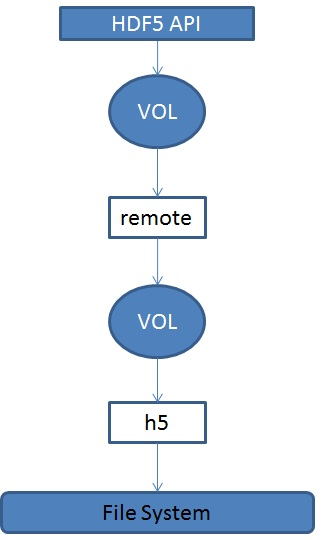
\includegraphics[width=90mm]{stacked.jpg}
\caption{Stacked VOL plugins.}
\label{stack}
\end{figure}

\subsection{Mirroring Plugins}
Another useful design option is to allow a mirroring plugin, where the
HDF5 API calls are forwarded through a mirror plugin to two or more
VOL plugins. This is an extention to the stacking
feature. Figure~\ref{mirror} shows an example of a VOL mirror that
maps HDF5 API calls to an h5 backend plugin and an XML backend plugin.

\begin{figure}[ht!]
\centering
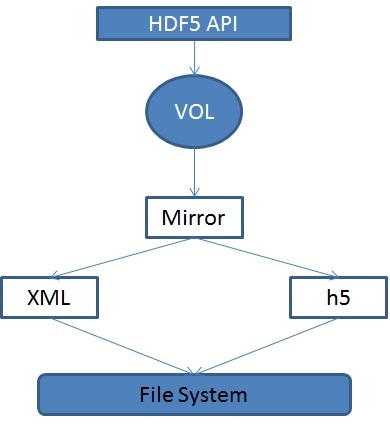
\includegraphics[width=90mm]{mirrored.jpg}
\caption{Mirrored VOL plugins.}
\label{mirror}
\end{figure}

Another possible VOL plugin could be a statistics plugin that just
gathers information on HDF5 API calls and records statistics
associated with the number of calls to a specific API functions and
corresponding parameters. This plugin would be very useful for
profiling purposes. The statistics plugin would be stacked on top of
another VOL plugin that actually performs the required access to the
file.

\subsection{Implementing Stacked and Mirrored Plugins}
A new set of API calls that map directly to the VOL callbacks have
been added to the HDF5 library to make stacking and mirroring easy for
plugin developers. Similarly to the public VFD (H5FD) routines that
call the VFD callbacks directly, we added the following H5VL APIs to
the library:

\begin{lstlisting}
/* ATTRIBUTE OBJECT ROUTINES */
void *H5VLattr_create(void *obj, H5VL_loc_params_t loc_params, H5VL_t *vol_plugin, const char *attr_name, hid_t acpl_id, hid_t aapl_id, hid_t dxpl_id, void **req);
void *H5VLattr_open(void *obj, H5VL_loc_params_t loc_params, H5VL_t *vol_plugin, const char *name, hid_t aapl_id, hid_t dxpl_id, void **req);
herr_t H5VLattr_read(void *attr, H5VL_t *vol_plugin, hid_t dtype_id, void *buf, hid_t dxpl_id, void **req);
herr_t H5VLattr_write(void *attr, H5VL_t *vol_plugin, hid_t dtype_id, const void *buf, hid_t dxpl_id, void **req);
herr_t H5VLattr_iterate(void *obj, H5VL_loc_params_t loc_params,
H5VL_t *vol_plugin, H5_index_t idx_type, H5_iter_order_t order,
hsize_t *n, H5A_operator2_t op, void *op_data, hid_t dxpl_id, void **req);
herr_t H5VLattr_get(void *attr, H5VL_t *vol_plugin, H5VL_attr_get_t get_type, hid_t dxpl_id, void **req, va_list arguments);
herr_t H5VLattr_remove(void *obj, H5VL_loc_params_t loc_params, H5VL_t
*vol_plugin, const char *attr_name, hid_t dxpl_id, void **req);
herr_t H5VLattr_close(void *attr, H5VL_t *vol_plugin, hid_t dxpl_id, void **req);

/* DATASE OBJECT ROUTINES */
void *H5VLdataset_create(void *obj, H5VL_loc_params_t loc_params,
H5VL_t *vol_plugin, const char *name, hid_t dcpl_id, hid_t dapl_id, hid_t dxpl_id, void **req);
void *H5VLdataset_open(void *obj, H5VL_loc_params_t loc_params, H5VL_t
*vol_plugin, const char *name, hid_t dapl_id, hid_t dxpl_id, void **req);
herr_t H5VLdataset_read(void *dset, H5VL_t *vol_plugin, hid_t
mem_type_id, hid_t mem_space_id, hid_t file_space_id, hid_t plist_id, void *buf, void **req);
herr_t H5VLdataset_write(void *dset, H5VL_t *vol_plugin, hid_t
mem_type_id, hid_t mem_space_id, hid_t file_space_id, hid_t plist_id, const void *buf, void **req);
herr_t H5VLdataset_set_extent(void *dset, H5VL_t *vol_plugin, const hsize_t size[], hid_t dxpl_id, void **req);
herr_t H5VLdataset_get(void *dset, H5VL_t *vol_plugin,
H5VL_dataset_get_t get_type, hid_t dxpl_id, void **req, va_list arguments);
herr_t H5VLdataset_close(void *dset, H5VL_t *vol_plugin, hid_t dxpl_id, void **req);

/* DATATYPE OBJECT ROUTINES */
void *H5VLdatatype_commit(void *obj, H5VL_loc_params_t loc_params, H5VL_t *vol_plugin, const char *name, hid_t type_id, hid_t lcpl_id, hid_t tcpl_id, hid_t tapl_id, hid_t dxpl_id, void **req);
void *H5VLdatatype_open(void *obj, H5VL_loc_params_t loc_params, H5VL_t *vol_plugin, const char *name, hid_t tapl_id, hid_t dxpl_id, void **req);
ssize_t H5VLdatatype_get_binary(void *obj, H5VL_t *vol_plugin, unsigned char *buf, size_t size, hid_t dxpl_id, void **req);
herr_t H5VLdatatype_get(void *obj, H5VL_t *vol_plugin, H5VL_datatype_get_t get_type, hid_t dxpl_id, void **req, va_list arguments);
herr_t H5VLdatatype_close(void *dt, H5VL_t *vol_plugin, hid_t dxpl_id,
void **req);

/* FILE OBJECT ROUTINES */
void *H5VLfile_create(H5VL_t **vol_plugin, const char *name, unsigned flags, hid_t fcpl_id, hid_t fapl_id, hid_t dxpl_id, void **req);
void *H5VLfile_open(H5VL_t **vol_plugin, const char *name, unsigned flags, hid_t fapl_id, hid_t dxpl_id, void **req);
herr_t H5VLfile_flush(void *obj, H5VL_loc_params_t loc_params, H5VL_t *vol_plugin, H5F_scope_t scope, hid_t dxpl_id, void **req);
herr_t H5VLfile_misc(void *file, H5VL_t *vol_plugin, H5VL_file_misc_t misc_type, hid_t dxpl_id, void **req, va_list arguments);
herr_t H5VLfile_optional(void *file, H5VL_t *vol_plugin,
H5VL_file_optional_t optional_type, hid_t dxpl_id, void **req, va_list arguments);
herr_t H5VLfile_get(void *file, H5VL_t *vol_plugin, H5VL_file_get_t get_type, hid_t dxpl_id, void **req, va_list arguments);
herr_t H5VLfile_close(void *file, H5VL_t *vol_plugin, hid_t dxpl_id, void **req);

/* GROUP OBJECT ROUTINES */
void *H5VLgroup_create(void *obj, H5VL_loc_params_t loc_params, H5VL_t
*vol_plugin, const char *name, hid_t gcpl_id, hid_t gapl_id, hid_t dxpl_id, void **req);
void *H5VLgroup_open(void *obj, H5VL_loc_params_t loc_params, H5VL_t
*vol_plugin, const char *name, hid_t gapl_id, hid_t dxpl_id, void
**req);
herr_t H5VLgroup_get(void *obj, H5VL_t *vol_plugin, H5VL_group_get_t get_type, hid_t dxpl_id, void **req, va_list arguments);
herr_t H5VLgroup_close(void *grp, H5VL_t *vol_plugin, hid_t dxpl_id, void **req);

/* LINK OBJECT ROUTINES */
herr_t H5VLlink_create(H5VL_link_create_type_t create_type, void *obj,
H5VL_loc_params_t loc_params, H5VL_t *vol_plugin, hid_t lcpl_id, hid_t
lapl_id, hid_t dxpl_id, void **req);
herr_t H5VLlink_move(void *src_obj, H5VL_loc_params_t loc_params1,
void *dst_obj, H5VL_loc_params_t loc_params2, H5VL_t *vol_plugin,
hbool_t copy_flag, hid_t lcpl_id, hid_t lapl_id, hid_t dxpl_id, void **req);
herr_t H5VLlink_iterate(void *obj, H5VL_loc_params_t loc_params,
H5VL_t *vol_plugin, hbool_t recursive, H5_index_t idx_type,
H5_iter_order_t order, hsize_t *idx, H5L_iterate_t op, void *op_data, hid_t dxpl_id, void **req);
herr_t H5VLlink_get(void *obj, H5VL_loc_params_t loc_params, H5VL_t
*vol_plugin, H5VL_link_get_t get_type, hid_t dxpl_id, void **req, va_list arguments);
herr_t H5VLlink_remove(void *obj, H5VL_loc_params_t loc_params, H5VL_t
*vol_plugin, hid_t dxpl_id, void **req);

/* OBJECT ROUTINES */
void *H5VLobject_open(void *obj, H5VL_loc_params_t loc_params, H5VL_t *vol_plugin, H5I_type_t *opened_type, hid_t dxpl_id, void **req);
herr_t H5VLobject_copy(void *src_obj, H5VL_loc_params_t loc_params1,
H5VL_t *vol_plugin1, const char *src_name, void *dst_obj,
H5VL_loc_params_t loc_params2, H5VL_t *vol_plugin2, const char *dst_name, hid_t ocpypl_id, hid_t lcpl_id, hid_t dxpl_id, void **req);
herr_t H5VLobject_visit(void *obj, H5VL_loc_params_t loc_params,
H5VL_t *vol_plugin, H5_index_t idx_type, H5_iter_order_t order, H5O_iterate_t op, void *op_data, hid_t dxpl_id, void **req);
herr_t H5VLobject_get(void *obj, H5VL_loc_params_t loc_params, H5VL_t
*vol_plugin, H5VL_object_get_t get_type, hid_t dxpl_id, void **req, va_list arguments);
herr_t H5VLobject_misc(void *obj, H5VL_loc_params_t loc_params, H5VL_t
*vol_plugin, H5VL_object_misc_t misc_type, hid_t dxpl_id, void **req, va_list arguments);
herr_t H5VLobject_optional(void *obj, H5VL_loc_params_t loc_params,
H5VL_t *vol_plugin, H5VL_object_misc_t optional_type, hid_t dxpl_id, void **req, va_list arguments);
herr_t H5VLobject_close(void *obj, H5VL_loc_params_t loc_params, H5VL_t *vol_plugin, hid_t dxpl_id, void **req);

/* ASYNCHRONOUS ROUTINES */
herr_t H5VLrequest_cancel(void **req, H5VL_t *vol_plugin, H5ES_status_t *status);
herr_t H5VLrequest_test(void **req, H5VL_t *vol_plugin, H5ES_status_t *status);
herr_t H5VLrequest_wait(void **req, H5VL_t *vol_plugin, H5ES_status_t *status);
\end{lstlisting}

The above API calls should be used in the stacked or mirror plugin to
call into the lower plugins indicated by the {\tt vol\_plugin}
parameter that is added to all the routines.

%%% Local Variables: 
%%% mode: latex
%%% TeX-master: t
%%% End: 


\end{document}